%%
%% Copyright (c) 2018-2019 Weitian LI <liweitianux@sjtu.edu.cn>
%% Creative Commons BY 4.0
%%

\acuse{colorbar}

\chapter{低频射电天空的模拟}
\label{chap:simulation}

为了能够评估射电晕对 EoR 探测的影响以及研发 EoR 信号分离算法,
首先需要进行低频射电天空的高精度模拟,包括 EoR 信号以及各种主要前景成分.
以我们之前的工作\cite{wang2010,wang2013}为基础,
我们开发了
\href{https://github.com/liweitianux/fg21sim}{\texttt{FG21sim}}\footnote{%
  FG21sim: \url{https://github.com/liweitianux/fg21sim}}
软件用来模拟主要的前景成分,
具体包括银河系的\ac{rad-syn}和\ac{rad-ff}、河外点源、以及星系团射电晕.
参考前人的相关研究 \cite{liu2009ps,datta2010,chapman2012,sims2016},
我们选取了三个常用的频带,分别为 \numrange{120}{128}、
\numrange{154}{162} 和 \numrange{192}{200} \si{\MHz}.
频带的宽度取为 \SI{8}{\MHz},这是为了限制宇宙的演化效应,
从而简化\ac{ps}的计算 (\autoref{sec:ps}) \cite{wyithe2004,thyagarajan2013}.
考虑到 SKA1-Low 在 \SI{120}{\MHz} 的视场大小 $\ac{Fov} \sim \SI{5}{\degree}$,
我们将模拟的天区大小设为 \SI{10 x 10}{\degree}.
此外,模拟的图像大小为 \num{1800 x 1800},即像素大小为 \SI{20}{\arcsecond}.
\autoref{tab:freq-bands} 汇总了这些模拟参数.

\begin{table}[htp]
  \centering
  \bicaption{%
    三个频带的模拟参数
  }{%
    Simulation Parameters for the Three Frequency Bands
  }
  \label{tab:freq-bands}

  \begin{tabular}{cccc}
    \toprule
    频段 &
      \SIrange{120}{128}{\MHz} &
      \SIrange{154}{162}{\MHz} &
      \SIrange{192}{200}{\MHz} \\
    \midrule
    中心频率 ($\nu_c$) & \SI{124}{\MHz} & \SI{158}{\MHz} & \SI{196}{\MHz} \\
    EoR 红移范围 &
      \numrange{10.10}{10.84} &
      \numrange{7.77}{8.22} &
      \numrange{6.10}{6.40} \\
    带宽 (\ac{bandwidth}) & \multicolumn{3}{c}{\SI{8}{\MHz}} \\
    天区坐标 & \multicolumn{3}{c}{%
      (R.A., Dec.\@) = (\SI{0}{\degree}, \SI{-27}{\degree})} \\
    天区大小 & \multicolumn{3}{c}{\SI{10 x 10}{\degree}} \\
    图像大小 & \multicolumn{3}{c}{\num{1800 x 1800}} \\
    像素大小 & \multicolumn{3}{c}{\SI{20}{\arcsecond}} \\
    \bottomrule
  \end{tabular}
\end{table}

本章首先重点阐述对星系团射电晕的建模及其结果 (\autoref{sec:simu-halos}),
接着介绍银河系 (\autoref{sec:simu-galactic})
和河外点源 (\autoref{sec:simu-eg-point}) 的模拟方法,
然后描述如何生成 EoR 信号的天图 (\autoref{sec:simu-eor}),
最后一节 (\autoref{sec:obs-simu}) 说明如何开展模拟观测并得到
SKA1-Low \enquote{观测}的图像.
通过将射电晕与其他前景成分(如银河系、河外点源)进行对比,
可以从另一个角度反映射电晕作为前景污染源的重要性.


%=====================================================================
\section{星系团射电晕}
\label{sec:simu-halos}

截至目前,只有少量几个工作在研究 EoR 前景时考虑了\ac{gc}\ac{rh}
\cite{diMatteo2004,gleser2008,jelic2008},
而且对\ac{rh}的建模过于简化,比如
直接使用在低流量端很不完备的 \SI{1.4}{\GHz} \ac{f-flux} \cite{gleser2008}、
采用弥散很大的射电--X 射线标度关系 \cite{jelic2008}、
假定相同的频谱指数和均匀的表面亮度分布 \cite{gleser2008,jelic2008}.

为了更加充分地评估\ac{rh}对 EoR 探测的具体影响,
有必要努力改进\ac{rh}的建模,获得更加逼真的\ac{rh}的图像和频谱信息.
为此,我们之前的一项工作\cite{wang2010}考虑了高能电子的能量损失过程,
改进了\ac{rh}的频谱特征的模拟.
在此基础上,本工作采用了一种半解析方法考虑了\ac{rh}的形成和演化过程,
进一步显著改进了\ac{rh}的建模.
对于一个\ac{gc},
首先根据扩展 Press--Schechter 理论
模拟其并合历史 (\autoref{sec:merging-history}),
然后运用\ac{turbreacc-model}来计算并合所产生的\ac{turbulence}对
\ac{icm} 中高能电子的再加速过程 (\autoref{sec:halo-evo}),
获得高能电子的能谱以及\ac{rh}的频谱随时间的演化 (\autoref{sec:numerical}),
从而得到所形成的\ac{rh}的性质 (\autoref{sec:halo-size})
并生成相应的图像 (\autoref{sec:halo-maps}).

Enrico Fermi 最早在 1949 年提出\ac{mfluid}中的带电粒子
可与其中的\ac{turbulence}发生随机散射而获得能量,
并用来解释高能\ac{cr}的起源 \cite{fermi1949,fermi1954,davis1956},
这个加速机制被称为\emph{二阶 Fermi 加速}.
\ac{gc} \ac{icm} 主要包含 $\gtrsim$\,\SI{1}{\keV} 的高温等离子气体,
同时还存在约 \si{\uG} 的磁场 \cite{govoni2004,ryu2008},所以是一个\ac{mfluid}.
为了解释\ac{rh}的性质(如尺度达 $\sim\si{Mpc}$、只在并合星系团中发现)和形成机制,
\citeay{brunetti2001} 和 \citeay{petrosian2001}
率先将二阶 Fermi 加速机制应用于\ac{gc} \ac{icm},
认为并合会产生大规模的\ac{turbulence},
就地加速 \ac{icm} 中的相对论性电子,
从而产生弥散的同步辐射,形成大尺度的\ac{rh}.
这就是\emph{\ac{turbreacc-model}}.
该模型在诸多后续研究中得到了充分的发展和改进
\cite{fujita2003,brunetti2004,cassano2005,brunetti2007,brunetti2011},
是目前解释\ac{rh}的主流模型.
详见 \citeay{brunetti2014} 综述文.
下文将详细介绍\ac{rh}的建模方法和结果.

%---------------------------------------------------------------------
\subsection{质量函数}
\label{sec:mass-function}

现在普遍认为,宇宙目前的结构是由极早期的微小密度扰动发展而来的 \cite{peebles1980}.
根据\acf{cdm} 模型,\ac{cdm} 粒子的速度弥散很小,因此有利于先形成小尺度结构;
然后在引力和宇宙膨胀的共同作用下,逐步形成尺度越来越大的结构
\cite{davis1985,bond1991,lacey1993}.
这就是\emph{\acf{hier-clustering}}模型.

当密度扰动进入非线性增长阶段,计算变得非常复杂而主要依赖于数值模拟.
\ac{spherical-collapse}模型可作为一个简单的解析近似,
能够给出与数值模拟相近的结果 \cite{gunn1972}.
根据该模型,暗物质坍缩形成暗物质晕,然后重子物质被暗物质晕的引力\ac{accretion},
在晕中沉积并演化为星系、星系团等结构.
利用这个模型,\citeay{press1974} 从密度扰动的随机统计性质推导出了暗物质晕
(即星系、星系团等结构)的数目随质量的分布及其时间演化,
即 \emph{Press-Schechter 质量函数}.
在红移 $z$ 处,每单位\ac{V-comoving}内质量范围为 $[M,\, M+\R{d}M]$
的\ac{gc}的数目 \ac{n-cl} 为:
\begin{equation}
  \label{eq:ps-mass-func}
  \ac{n-cl} \,\D{M} =
    \sqrt{\frac{2}{\Cpi}} \frac{\langle \rho_0 \rangle}{M}
    \frac{\delta_c(z)}{\sigma^2(M)} \left| \diff{\sigma(M)}{M} \right|
    \exp\!\left[ -\frac{\delta_c^2(z)}{2\sigma^2(M)} \right] \,\D{M} ,
\end{equation}
其中
$M$ 是星系团的质量,
$\langle \rho_0 \rangle$ 是当前的宇宙平均密度,
$\delta_c(z)$ 是暗物质坍缩形成暗物质晕的\acl{delta-crit}
(critical linear overdensity) [见\autoref{eq:delta-crit}],
$\sigma(M)$ 是当前在平均质量为 $M$ 的球形区域里的密度涨落的\ac{rms}值.

在星系团的质量范围内,上式中的密度涨落 $\sigma(M)$ 可合理地近似为以下幂律形式
\cite{sarazin2002,randall2002}:
\begin{equation}
  \label{eq:sigma-mass}
  \sigma(M) = \ac{sigma8} \left( \frac{M}{M_8} \right)^{-\alpha} ,
\end{equation}
其中
\ac{sigma8} 是\acl{sigma8},
$M_8$ 是半径为 \SI{8}{\per\hubble\Mpc} 的球形区域里的质量:
\begin{equation}
  M_8 = \frac{4\Cpi \langle \rho_0 \rangle}{3}
    (\SI{8}{\per\hubble\Mpc})^3 ,
\end{equation}
以及指数 $\alpha = (n+3)/6$ 并且有 $n = -7/5$ \cite{bahcall1998}.

设星系团的质量下限为 $M_{\R{min}} = \SI{2e14}{\solarmass}$
以及红移上限为 $z_{\R{max}} = 4$,
于是由 Press--Schechter 质量函数 [\autoref{eq:ps-mass-func}]
可计算出 \SI{10 x 10}{\degree} 的天区内的星系团总数为 504,
以及相应的质量和红移分布(如\autoref{fig:m-z-dist} 所示).
接着,对质量和红移分布随机采样,得到一系列 $(M_{\R{sim}}, z_{\R{sim}})$ 对,
于是构建成所需的星系团样本.

\begin{figure}[htp]
  \centering
  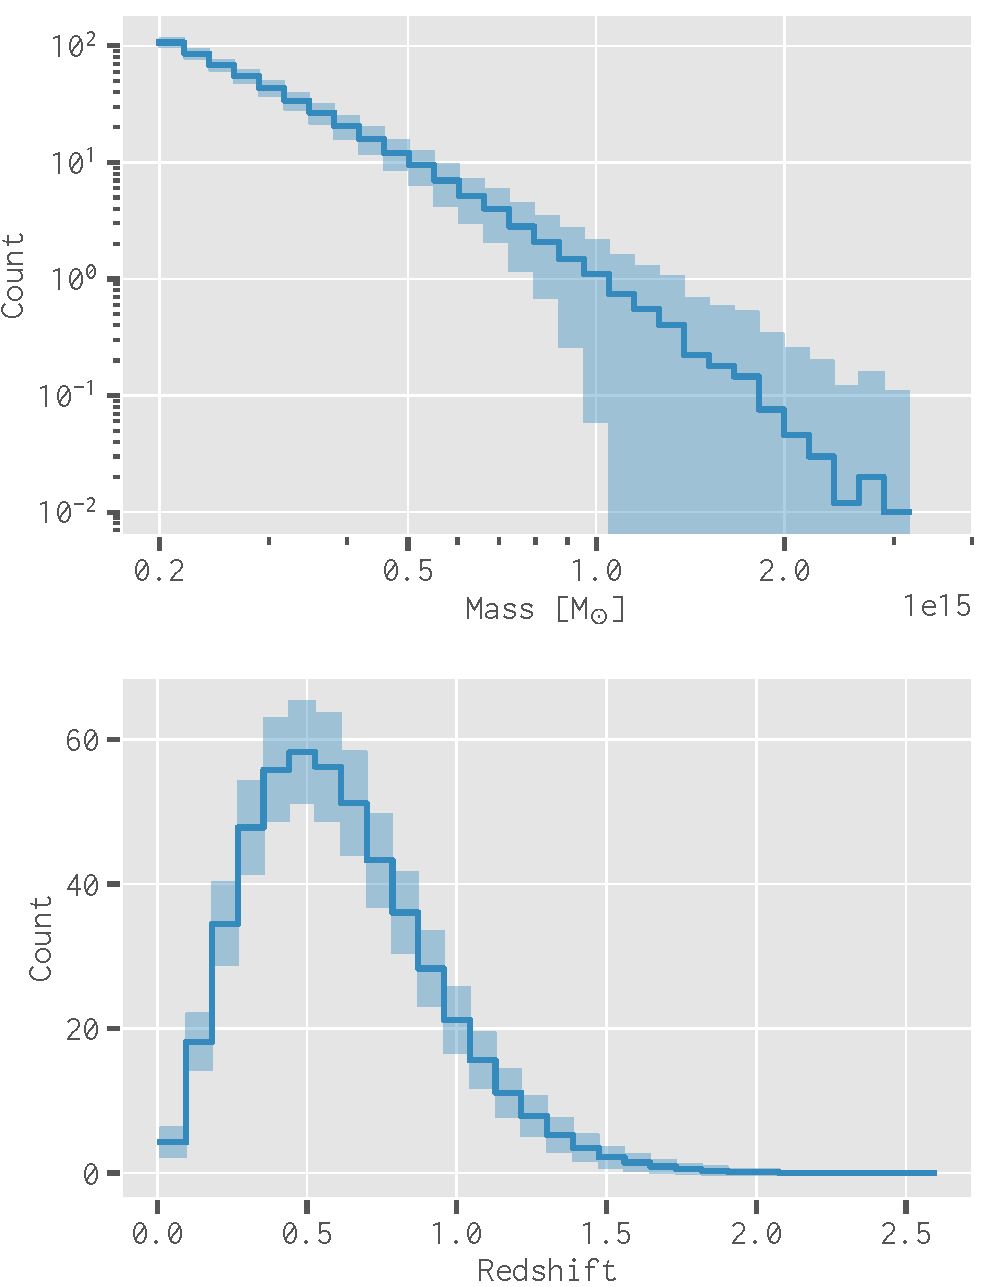
\includegraphics[width=0.8\textwidth]{mass-z-dist}
  \bicaption[星系团的红移和质量分布直方图]{%
    在 \SI{10 x 10}{\degree} 的天区内,星系团的红移(上栏)和质量(下栏)分布直方图.
    图中的实线和阴影区域分别表示 500 次模拟的平均值和 68\% 的误差.
  }{%
    The mass (upper panel) and redshift (lower panel) histograms of the
    simulated galaxy clusters in a \SI{10 x 10}{\degree} sky patch.
    The solid lines and shaded regions represent the means and
    68\% uncertainties derived from 500 simulation runs,
    respectively.
  }
  \label{fig:m-z-dist}
\end{figure}

%---------------------------------------------------------------------
\subsection{并合历史}
\label{sec:merging-history}

上述 Press--Schechter 质量函数只给出了在不同红移处宇宙中的\ac{gc}的质量分布,
没有提供单个星系团的形成历史.
这个问题由 \citeay{lacey1993} 通过拓展 Press--Schechter 理论而给出了一个解决方案.
给定一个星系团,扩展 Press--Schechter 理论描述了其\ac{progenitor}的质量分布规律,
然后利用 Monte Carlo 模拟便可构建出该星系团的成长历史,即\emph{\acf{m-tree}}
\cite{lacey1993,randall2002}.

设一个星系团在 $t_1$ 时刻的质量为 $M_1$,经过一次成长步骤(并合或\ac{accretion})后,
其质量在 $t_2$ ($> t_1$) 时刻增长为 $M_2$.
给定 $M_2$ 和 $t_2$,扩展 Press--Schechter 理论给出了该星系团在一个较早时刻 $t_1$
具有一个质量范围为 $[M_1,\, M_1+\D{M_1}]$ 的\ac{progenitor}的\ac{pr-cond}为
\cite{lacey1993,randall2002}:
\begin{equation}
  \label{eq:eps-condprob}
  \R{Pr}(M_1, t_1 \,|\, M_2, t_2) \,\D{M_1} =
    \frac{1}{\sqrt{2\Cpi}} \frac{M_2}{M_1}
    \frac{\delta_{c1} - \delta_{c2}}{(\sigma_1^2 - \sigma_2^2)^{3/2}}
    \left| \diff{\sigma_1^2}{M_1} \right|
    \exp \!\left[ -\frac{(\delta_{c1} - \delta_{c2})^2}
      {2(\sigma_1^2 - \sigma_2^2)} \right] \,\D{M_1} ,
\end{equation}
其中
$\delta_{ci} \equiv \delta_c(t_i)$,$\sigma_i \equiv \sigma(M_i)$,
同时下标 $i = 1, 2$ 分别表示这两个参数在时刻 $t_1$ 和 $t_2$ 的值.
进一步定义 $\psi \equiv \sigma^2(M)$ 和 $\omega \equiv \delta_c(t)$,
上式可简化为:
\begin{equation}
  \label{eq:eps-condprob2}
  \R{Pr}(\Delta\psi, \Delta\omega) \,\D{\Delta\psi} =
    \frac{1}{\sqrt{2\Cpi}} \frac{\Delta\omega}{(\Delta\psi)^{3/2}}
    \exp \!\left[ -\frac{(\Delta\omega)^2}{2 \Delta\psi} \right]
    \,\D{\Delta\psi} ,
\end{equation}
其中
$\Delta\psi = \sigma_1^2 - \sigma_2^2$,
$\Delta\omega = \delta_{c1} - \delta_{c2}$.
注意,$\psi$ 随 $M$ 的增大而单调递减,$\omega$ 随 $t$ 的增大而单调递减.

对于 \autoref{sec:mass-function} 样本中的每一个星系团,为了模拟其\ac{m-tree},
我们从\enquote{当前的}质量 $M_{\R{sim}}$ 和红移 $z_{\R{sim}}$ 出发,
运用 Monte Carlo 方法逐步追溯其成长历史,时间步长为 $\Delta\omega$.
为了能够分辨质量变化为 $\Delta M_c$ ($\ll M_2$) 的并合,
时间步长 $\Delta\omega$ 应满足 \cite{lacey1993}:
\begin{equation}
  \Delta\omega \lesssim (\Delta\omega)_{\R{max}} =
    \left[ \psi \left| \diff{\ln \sigma^2}{\ln M_2} \right|
      \left( \frac{\Delta M_c}{M_2} \right) \right]^{1/2} .
\end{equation}
我们采用了自适应的时间步长 \cite{randall2002}:
$\Delta\omega = (\Delta\omega)_{\R{max}} \big/ 2$.

在追溯的每一步,当时间步长 $\Delta\omega$ 确定后,
则并入星系团的质量(由 $\Delta\psi$ 描述)的\ac{cdf}为:
\begin{align}
  F_{\Delta\psi}(<\!\Delta\psi, \Delta\omega)
    & = \int_0^{\Delta\psi} \R{Pr}(\Delta\psi', \Delta\omega)
      \,\D{\Delta\psi'} \\
    & = 1 - \erf \left( \frac{\Delta\omega}{\sqrt{2\Delta\psi}} \right) ,
  \label{eq:cdf-submass}
\end{align}
其中 $\erf(\cdot)$ 为\ac{errfunc}:
\begin{equation}
  \erf(x) = \frac{2}{\sqrt{\pi}} \int_0^x \Ce^{-t^2} \,\D{t} .
\end{equation}
对\autoref{eq:cdf-submass} 随机采样得到一个 $\Delta\psi$,
于是,星系团 $M_2$ 的一个\ac{progenitor}的质量 $M_1$
由 $\psi_1 = \psi_2 + \Delta\psi$ 确定 [参见\autoref{eq:sigma-mass}],
同时另一个\ac{progenitor}的质量为 $\Delta M = M_2 - M_1$.
设 $M_m \equiv \max(M_1, \Delta M)$ 和 $M_s \equiv \min(M_1, \Delta M)$
分别为并合的主星系团(简称\emph{主团})和子星系团(简称\emph{子团})的质量,
如果 $M_s > \Delta M_c$,则认为发生了一次并合事件,
否则认为是\ac{accretion}过程 \cite{randall2002}.

目前普遍认为可观测到的\ac{rh}与最近(在观测者的参考系)发生的\ac{m-major}密切相关,
而且\ac{rh}的典型寿命较短,比如在 \SI{1.4}{\GHz} 的寿命
$\tau_{\R{halo}} \lesssim \SI{1}{\Gyr}$ \cite{brunetti2009,cassano2016}.
因此,我们采用 $\Delta M_c = \SI{e13}{\solarmass}$ \cite{cassano2005},
并且只针对主团从\enquote{当前}时刻 $t_{\R{sim}}$ (对应于 $z_{\R{sim}}$)
追溯 $t_{\R{back}} = \SI{3}{\Gyr}$.
这样,我们获得了每个星系团的并合历史
$\left\{\left( M_m^{(i)}, M_s^{(i)}, t_{\R{merger}}^{(i)} \right)\right\}$
用于开展后续的射电晕的模拟.

星系团的并合历史(即\ac{m-tree})是随机模拟的.
以一个质量为 \SI{e15}{\solarmass} 的星系团为例,重复模拟其\ac{m-tree} 30 次,
得到的 30 颗\ac{m-tree}互不相同,如\autoref{fig:merging-history} 上栏所示.
同时,该图下栏显示了从 \autoref{sec:mass-function} 样本中随机挑选的 30 个星系团
的\ac{m-tree},其中每个星系团只随机生成了一颗\ac{m-tree}.

\begin{figure}[htp]
  \centering
  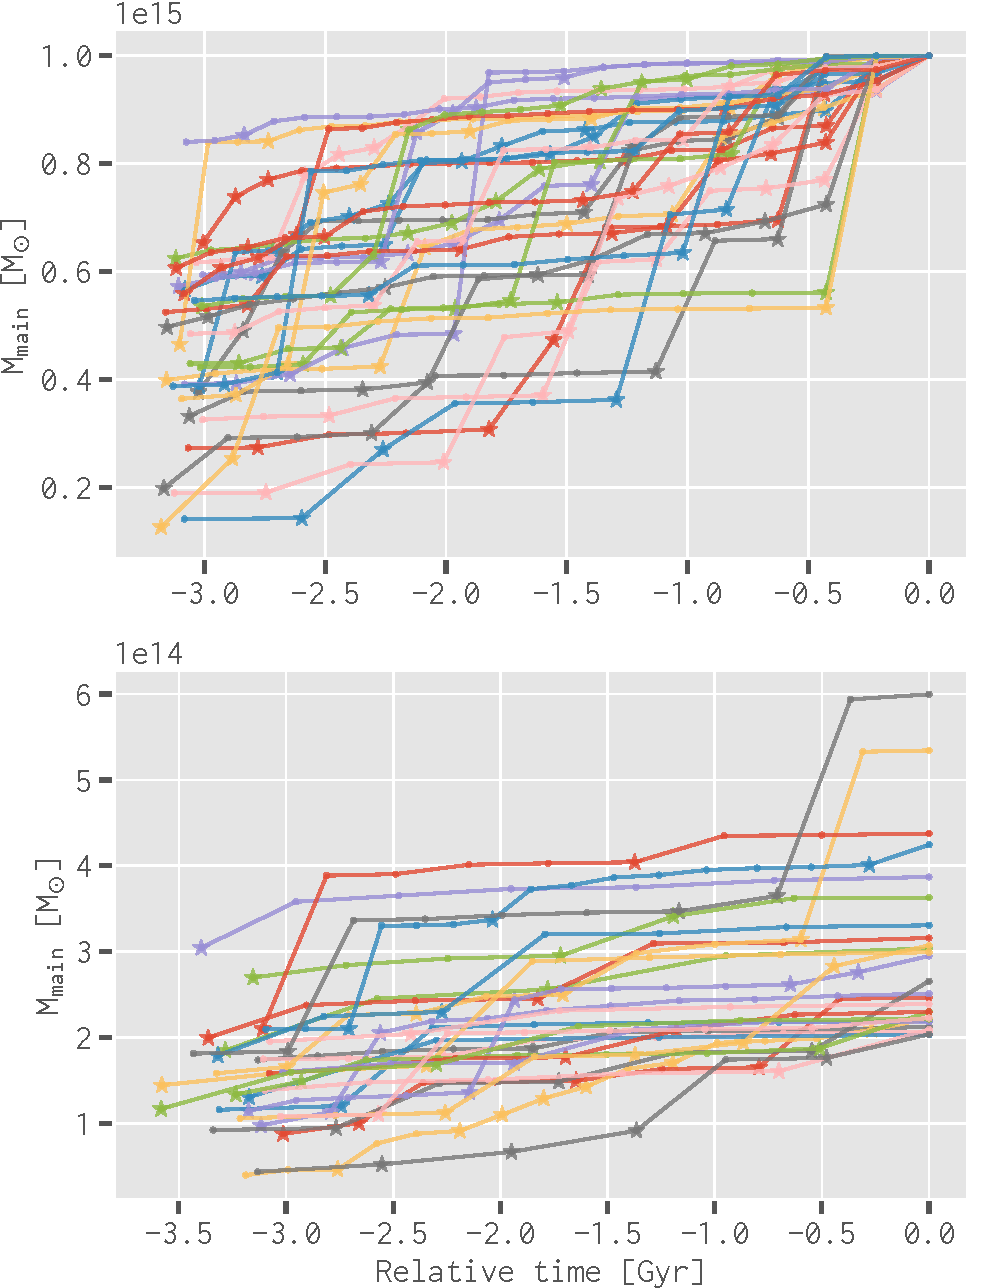
\includegraphics[width=0.8\textwidth]{merging-history}
  \bicaption[星系团并合树的模拟结果示例]{%
    \uline{(上栏)}
    对同一个质量为 \SI{e15}{\solarmass} 的星系团,重复模拟其\acs*{m-tree} 30 次
    所得到的 30 颗不同的\acs*{m-tree}.
    \uline{(下栏)}
    从 \autoref{sec:mass-function} 样本中随机挑选 30 个星系团,
    对每个星系团随机模拟一颗\acs*{m-tree}.
    星号和圆点分别表示并合和\acs*{accretion}事件.
  }{%
    \textbf{(Upper)} Merger trees for one galaxy cluster of mass
    \SI{e15}{\solarmass} obtained by repeating the random build process
    for 30 times.
    \textbf{(Lower)} Example merger trees for 30 galaxy clusters randomly
    drawn from the sample constructed in \autoref{sec:mass-function}.
    Asterisks mark merger events and dots represent accretion events.
  }
  \label{fig:merging-history}
\end{figure}

%---------------------------------------------------------------------
\subsection{演化模型}
\label{sec:halo-evo}

根据\ac{turbreacc-model},星系团 \ac{icm} 里充满一群非热的\ac{e-primary},
这些电子可在多种过程中产生并被注入到 \ac{icm} 中,比如 \ac{agn} 活动、恒星形成,
详见 \citeay{blasi2007} 和 \citeay{brunetti2014} 综述文.
当星系团经历\ac{m-major}时,整个 \ac{icm} 中都将产生剧烈的\ac{turbulence},
就地加速\ac{e-primary}至极高的能量 (\acl{g} $\ac{g} > \num{e3}$),
从而形成弥散的\ac{rh}.
在另一方面,多种机制会使这些高能电子损失能量 \cite{sarazin1999},其中包括:
产生\ac{rad-syn}、与 \ac{cmb} 光子发生逆 Compton 散射、
与 \ac{icm} 中的离子发生 Coulomb 碰撞.

对于一群能量分布各向同性的电子,在上述加速和能量损失的共同作用,
其能谱 \ac{n-e} 随时间的演化由以下 Fokker--Planck 方程描述
\cite{eilek1991,schlickeiser2002}:
\begin{equation}
  \label{eq:fokkerplanck}
  \pdiff{\ac{n-e}}{t} =
    \pdiff{}{\ac{g}} \left[ \ac{n-e} \left(
      \left| \diff{\ac{g}}{t} \right| -
      \frac{2}{\ac{g}} \ac{coef-diffusion}(\ac{g}, t) \right) \right]
    + \pdiff{}{\ac{g}} \left[
      \ac{coef-diffusion} \pdiff{\ac{n-e}}{\ac{g}} \right]
    + \ac{e-inj}(\ac{g}, t) ,
\end{equation}
其中
\ac{coef-diffusion} 是描述\ac{turbulence}和电子相对作用的\acl{coef-diffusion},
$|\R{d}\gamma / \R{d}t|$ 是电子的能量损失速率,
还有 \ac{e-inj} 描述了电子的注入过程.

%.....................................................................
\subsubsection{热成分的性质}

对于星系团 \ac{icm} 的热成分,其中的热电子的数密度 (number density) \ac{n-th} 为:
\begin{equation}
  \label{eq:n-th}
  \ac{n-th} \simeq
    \frac{3 \ac{f-gas} \ac{M-vir}}{
      4\Cpi \ac{mol-weight-m} \ac{mass-u} \,r^3_{\R{vir}}} ,
\end{equation}
其中
$\ac{mol-weight-m} \simeq 0.6$ 是 \ac{icm} 的\acl{mol-weight-m}
(mean molecular weight) \cite{ettori2013},
\ac{mass-u} 是\acl{mass-u} (atomic mass unit),
\ac{M-vir} 是星系团的\acl{M-vir} (virial mass),
\ac{r-vir} 是其\acl{r-vir} (virial radius)
[参见\autoref{eq:radius-virial}],
以及 $\ac{f-gas} \simeq \ac{Ob0}/\ac{Om0}$
是星系团中的气体质量占总质量 (\ac{M-vir}) 的比例.

于是,\ac{icm} 的热能密度 (thermal energy density) \ac{e-th} 由下式给出:
\begin{equation}
  \label{eq:e-th}
  \ac{e-th} = \frac{3}{2} \,\ac{n-th} \ac{kb} \ac{T-cl} ,
\end{equation}
其中 \ac{icm} 的平均温度 \ac{T-cl} 可近似为 \cite{cavaliere1998}:
\begin{equation}
  \label{eq:t-icm}
  \ac{T-cl} \simeq \ac{T-vir} + \frac{3}{2} \,T_{\R{out}} ,
\end{equation}
其中 \ac{T-vir} 为星系团的\acl{T-vir} (virial temperature):
\begin{equation}
  \ac{T-vir} =
    \frac{\ac{mol-weight-m} \ac{mass-u} \ac{G} \ac{M-vir}}{2\,\ac{r-vir}} ,
\end{equation}
以及 $T_{\R{out}} \simeq \SI{0.5}{\keV}$
是从星系团外围区域 ($\gtrsim \ac{r-vir}$) 流入的气体的温度 \cite{fujita2003}.

%.....................................................................
\subsubsection{电子注入过程}

在星系团及其成员星系中持续发生着 \ac{agn} 活动、恒星形成等过程,
不断地将\ac{e-primary}注入到 \ac{icm} 之中.
因此,可以假定\ac{e-primary}的注入速率 \ac{e-inj-rate} 是恒定的
\cite{cassano2005,donnert2014},
同时还可假定注入电子的能谱为幂律形式 \cite{sarazin1999},
于是注入电子的能谱为:
\begin{equation}
  \label{eq:electron-inj}
  \ac{e-inj}(\ac{g}, t)
    \simeq \ac{e-inj}(\ac{g})
    = \ac{e-inj-rate} \,\ac{g}^{-s} ,
\end{equation}
其中 $s$ 为谱指数,在本文中取为 2.5 \cite{cassano2005}.

进一步假定注入电子的总能量密度与 \ac{icm} 热能密度 \ac{e-th} 之比为
\ac{f-injection} \cite{cassano2005},即:
\begin{equation}
  \tau_{\R{cl}} \int_{\ac{g}_{\R{min}}}^{\ac{g}_{\R{max}}}
  \ac{e-inj}(\ac{g}') \,\ac{g}'\ac{e-electron} \,\D{\ac{g}'}
    = \ac{f-injection} \,\ac{e-th} ,
\end{equation}
其中
$\tau_{\R{cl}} \simeq t_{\R{sim}}$
(对应于红移 $z_{\R{sim}}$)是星系团\enquote{当前的}年龄,
$\ac{e-electron} = \ac{mass-e} \ac{speed-light}^2$
是\acl{e-electron} (rest energy).
考虑到 $\ac{g}_{\R{min}} \ll \ac{g}_{\R{\max}}$,
可推导出电子的注入速率 \ac{e-inj-rate} 为:
\begin{equation}
  \label{eq:injrate}
  \ac{e-inj-rate} \simeq
    \frac{(s-2)\,\ac{f-injection}\,\ac{e-th}}{
      \ac{e-electron}\,\tau_{\R{cl}}} \ac{g}_{\R{min}}^{s-2} .
\end{equation}

%.....................................................................
\subsubsection{剥离半径}

当一个子团并入主团时,其外围区域的气体将被\ac{ram-pressure}剥离,
即\emph{\acf{ram-pressure-strip}}效应 \cite{gunn1972}.
对子团而言,距离自身的中心越远,则气体的流体静力学压强越小,
\ac{ram-pressure-strip}的效果也就越显著.
因此\emph{\acl{r-strip} (stripping radius)} \ac{r-strip} 定义为,
该半径处子团受到的\ac{ram-pressure}与自由气体的流体静力学压强达到平衡
\cite{cassano2005},即:
\begin{equation}
  \label{eq:rs-eqp}
  \bar{\rho}_m v_{\R{imp}}^2
    = \frac{\ac{rho-s}(\acs{r-strip})}{\ac{mol-weight-m} \ac{mass-u}}
      \ac{kb} \ac{T-cl-s} ,
\end{equation}
其中
$\bar{\rho}_m = \ac{mol-weight-m} \ac{mass-u} \ac{n-th-m}$
是主团的平均气体密度,
\ac{v-imp} 是主团和子团之间的\acl{v-imp},
$\ac{rho-s}(r)$ 和 \ac{T-cl-s} 分别是子团的气体密度轮廓和 \ac{icm} 平均温度.

两个质量分别为 \ac{M-vir-m} 和 \ac{M-vir-s} 的星系团
从相距 $d_0$ 的地方以零初速度开始并合,
则两者的\acl{v-imp} \ac{v-imp} 为 \cite{sarazin2002,cassano2005}:
\begin{equation}
  \label{eq:v-imp}
  \ac{v-imp} \simeq \left[
    \frac{2 \ac{G} (\ac{M-vir-m} + \ac{M-vir-s})}{\ac{r-vir-m}}
    \left( 1 - \frac{1}{\eta_v} \right)\right]^{1/2} ,
\end{equation}
其中
\ac{r-vir-m} 为\acl{r-vir-m},
$\eta_v$ 为初始距离参数,由下式给出:
\begin{equation}
  \eta_v
    = \frac{d_0}{\ac{r-vir-m}}
    \simeq 4 \left( 1 + \frac{\ac{M-vir-s}}{\ac{M-vir-m}} \right)^{1/3} .
\end{equation}

星系团的气体密度轮廓可以很好地由 β 模型 \cite{cavaliere1976} 来描述:
\begin{equation}
  \label{eq:beta-model}
  \rho(r)
    = \rho(0) \left[ 1 + \left(
      \frac{r}{\ac{r-core}} \right)^2 \right]^{-3\ac{beta-slope}/2} ,
\end{equation}
其中
$\rho(0)$ 为中心处的气体密度,
\ac{r-core} 为\acl{r-core} (core radius),
\ac{beta-slope} 为\acl{beta-slope} (slope parameter).
本文选取了 $\ac{r-core} = 0.1 \,\ac{r-vir}$ \cite{sanderson2003}
以及 $\ac{beta-slope} = 2/3$ \cite{jones1984}.
将 β 模型应用于上述子团,于是有:
\begin{equation}
  \ac{rho-s}(r)
    = \ac{rho-s}(0) \left[ 1 + \left(
      \frac{r}{\ac{r-core-s}} \right)^2 \right]^{-3\ac{beta-slope}/2} ,
\end{equation}
其中
$\ac{r-core-s} = 0.1 \,\ac{r-vir-s}$,
以及 $\ac{rho-s}(0)$ 由子团的气体质量确定:
\begin{align}
  \ac{M-gas-s}
    & = \ac{f-gas} \ac{M-vir-s}
      = \int_0^{\ac{r-vir-s}} \ac{rho-s}(r) \,\D{r}  \\
    & = \ac{rho-s}(0) \int_0^{\ac{r-vir-s}}
        \left[ 1 + (r / \ac{r-core-s})^2 \right]^{-3\ac{beta-slope}/2}
        \,\D{r} .
\end{align}

%.....................................................................
\subsubsection{湍流加速}

在星系团 \ac{icm} 中,\ac{turbulence}与热成分粒子以及\ac{cr}等非热成分粒子
之间的相互作用非常复杂.
然而,我们目前对这些相互作用的具体细节及其微观物理机制的理解程度仍然非常有限.
详见 \citeay{lazarian2012}、\citeay{petrosian2012}、
\citeay{brunetti2014} 等综述文.

在多种由\ac{turbulence}引起的粒子加速机制中,最重要的一种机制是\emph{\acf{ttd}},
即\ac{turbulence}通过与 \ac{icm} 中的\ac{cr}等相对论性粒子发生相互作用而耗散能量,
从而将能量传递给电子使其加速
(参考 \citeay{brunetti2007} 和 \citeay{brunetti2011} 及其所引文献).
该加速机制给出\autoref{eq:fokkerplanck}
中的\acl{coef-diffusion} \ac{coef-diffusion} 为
\cite{miniati2015,pinzke2017}:
\begin{equation}
  \ac{coef-diffusion}
    = 2\,\ac{g}^2 \ac{f-instability} \,\ac{k-turb-inj}
      \frac{\ac{v-turb}^2}{\ac{f-cr} \,c_s^3} ,
\end{equation}
其中
\ac{f-instability} 是描述 \ac{icm} 等离子体的不稳定性的参数,
$\ac{f-cr} = \epsilon_{\R{cr}} / \ac{e-th}$
是\ac{cr}的能量密度与 \ac{icm} 热能密度之比,
$\ac{k-turb-inj} \simeq 2\Cpi / \ac{r-turb}$
是\acl{k-turb-inj} (injection scale),
同时 \ac{r-turb} 是\acl{r-turb},
\ac{v-turb} 是\acl{v-turb} (velocity dispersion),
以及 \ac{speed-sound} 为 \ac{icm} 中的声速,由下式给出:
\begin{equation}
  \ac{speed-sound}
    = \sqrt{\frac{\ac{adiabatic-index} \ac{kb} \ac{T-cl}}{
        \ac{mol-weight-m} \ac{mass-u}}} ,
\end{equation}
其中 \ac{adiabatic-index} 是气体的\acl{adiabatic-index} (adiabatic index).
对于理想的单原子气体,$\ac{adiabatic-index} = 5/3$.

除并合之外,\ac{agn} 喷流、\ac{galactic-wind} 等过程也会在 \ac{icm}
中产生\ac{turbulence} \cite{vazza2011}.
\citeay{vazza2011} 发现在弛豫星系团的中央区域,
\ac{turbulence}的能量与 \ac{icm} 热能之比可达 $\lesssim\,$5\%.
因此,在并合开始前,\ac{turbulence}具有初始的速度弥散 \ac{v-turb0}:
\begin{equation}
  \label{eq:v-turb0}
  \ac{v-turb0}
    = 3 \,\ac{f-turb} \frac{\ac{kb} \ac{T-cl-m}}{
        \ac{mol-weight-m} \ac{mass-u}} ,
\end{equation}
其中
\ac{f-turb} 是初始湍流的能量密度与 \ac{icm} 热能密度 \ac{e-th} 之比.
并合会贡献一部分能量到\ac{turbulence}中,
使得\ac{turbulence}的速度弥散 \ac{v-turb} 显著增大,于是有:
\begin{align}
  \label{eq:energy-turb}
  E_{\R{turb}}
    & = \frac{1}{2} \ac{M-turb} \ac{v-turb}  \\
    & = \frac{1}{2} \ac{M-turb} \ac{v-turb0} + \ac{f-trans} E_m ,
\end{align}
% XXX: 'align' environment causes acro symbols not been printed in the list...
\acuse{M-turb,f-trans}
其中
$E_m$ 是子团在并合过程中释放的能量,
\ac{f-trans} 是并合注入湍流的能量比例,
以及 \ac{M-turb} 是半径为 \ac{r-turb} 的湍流区域内的气体质量,由下式给出:
\begin{equation}
  \ac{M-turb} = \int_0^{\ac{r-turb}} \! \rho(r) \,4\Cpi r^2 \,\D{r} ,
\end{equation}
其中 $\rho(r)$ 是已并合星系团的气体密度轮廓,同样由 β 模型描述
[参见\autoref{eq:beta-model}].
并合释放的能量 $E_m$ 可以近似为落入子团所做的功 \cite{fujita2003,cassano2005}:
\begin{equation}
  \label{eq:energy-inj}
  E_m \simeq \bar{\rho}_m v_{\R{imp}}^2 V_{\R{turb}} ,
\end{equation}
其中 $V_{\R{turb}}$ 为子团扫过的体积:
\begin{equation}
  V_{\R{turb}} \simeq \Cpi r_s^2 \,\ac{r-vir-m} .
\end{equation}
综上可得,在并合过程中,湍流的速度弥散 \ac{v-turb} 为:
\begin{equation}
  \ac{v-turb}
    = \ac{v-turb0}
    + 2 \Cpi\,\ac{f-trans}\, \bar{\rho}_m \ac{r-vir-m}
      \,\frac{r_s^2 v_{\R{imp}}^2}{\ac{M-turb}} .
\end{equation}

最后还需要估算\acl{r-turb} \ac{r-turb},我们假定了以下关系:
\begin{equation}
  \label{eq:r-turb}
  \ac{r-turb} \simeq \ac{r-strip} + \ac{r-core-m} ,
\end{equation}
其中
$\ac{r-core-m} = 0.1 \,\ac{r-vir-m}$ 是主团的\acl{r-core},
\ac{r-strip} 是落入子团的\acl{r-strip} [参见\autoref{eq:rs-eqp}].
对于\ac{m-major} ($\ac{M-vir-m} / \ac{M-vir-s} \lesssim 3$),
\acl{r-strip} \ac{r-strip} 约为 $\numrange{1}{2} \,\ac{r-core-m}$;
对于\ac{m-minor} ($\ac{M-vir-m} / \ac{M-vir-s} \sim \numrange{3}{10}$),
则有 $\ac{r-strip} < \ac{r-core-m}$.
前人的数值模拟研究显示,并合能够在半径约为 $\numrange{0.1}{0.3} \,r_{\R{vir,m}}$
的范围内产生显著的湍流 \cite{vazza2011,vazza2012,miniati2015ss}.
因此,我们计算的\acl{r-turb} \ac{r-turb} [\autoref{eq:r-turb}]
能够与这些模拟结果符合得比较好.
\autoref{eq:r-turb} 还显示,
\ac{m-minor}亦能在一个半径 $\gtrsim \ac{r-core-m}$ 的较大区域内产生湍流,
因为落入的子团会引起主团中央区域的气体\ac{sloshing},从而产生较大范围的湍流
\cite{vazza2012}.
尽管如此,\ac{m-minor}释放的能量 $E_m$ 明显少于\ac{m-major}
[参见\autoref{eq:energy-inj}],
因此产生的湍流也要弱很多.

%.....................................................................
\subsubsection{能量损失过程}

在\ac{gc} \ac{icm} 中,高能电子可通过多种机制损失能量 \cite{sarazin1999},
本文考虑了其中三种主要的机制.
第一种能量损失机制为高能电子与 \ac{cmb} 光子发生逆 Compton 散射,
对应的能量损失速率为:
\begin{equation}
  \label{eq:eloss-ic}
  \left( \diff{\ac{g}}{t} \right)_{\R{IC}} =
    \num{-4.32e-4} \,\ac{g}^2 (1+z)^4
    \quad [\si{\per\Gyr}] .
\end{equation}

第二,由于 \ac{icm} 中存在强度约 \si{\uG} 的磁场 \cite{govoni2004,ryu2008},
因此高能电子将产生\ac{rad-syn}而损失能量,该过程的能量损失速率为:
\begin{equation}
  \label{eq:eloss-syn}
  \left( \diff{\ac{g}}{t} \right)_{\R{syn}} =
    \num{-4.10e-5} \,\ac{g}^2
    \left( \frac{\ac{mag-field}}{\SI{1}{\uG}} \right)^2
    \quad [\si{\per\Gyr}] ,
\end{equation}
其中 \ac{mag-field} 是磁场强度,
并且假定 \ac{icm} 中的磁场强度是均匀的.
为了估算 \ac{mag-field} 的大小,可以利用一个常用的假设:
磁场与\ac{cr}达到能量\ac{equipartition} \cite{beck2005},
即两者的能量密度相等:
\begin{equation}
  \epsilon_B = \frac{\ac{mag-field}^2}{8\Cpi}
    \simeq \epsilon_{\R{cr}} = \ac{f-cr}\,\ac{e-th} .
\end{equation}

第三,高能电子与 \ac{icm} 中的热电子发生 Coulomb 碰撞而损失能量,
对应的能量损失速率为:
\begin{equation}
  \label{eq:eloss-coul}
  \left( \diff{\ac{g}}{t} \right)_{\R{Coul}} =
    \num{-3.79e4} \left( \frac{\ac{n-th}}{\SI{1}{\per\cm\cubed}} \right)
    \left[ 1 + \frac{1}{75} \ln \left(
        \ac{g}\,\frac{\SI{1}{\per\cm\cubed}}{\ac{n-th}} \right) \right]
    \quad [\si{\per\Gyr}] ,
\end{equation}
其中 \ac{n-th} 为热电子的数密度,由\autoref{eq:n-th} 给出.

\begin{figure}[htp]
  \centering
  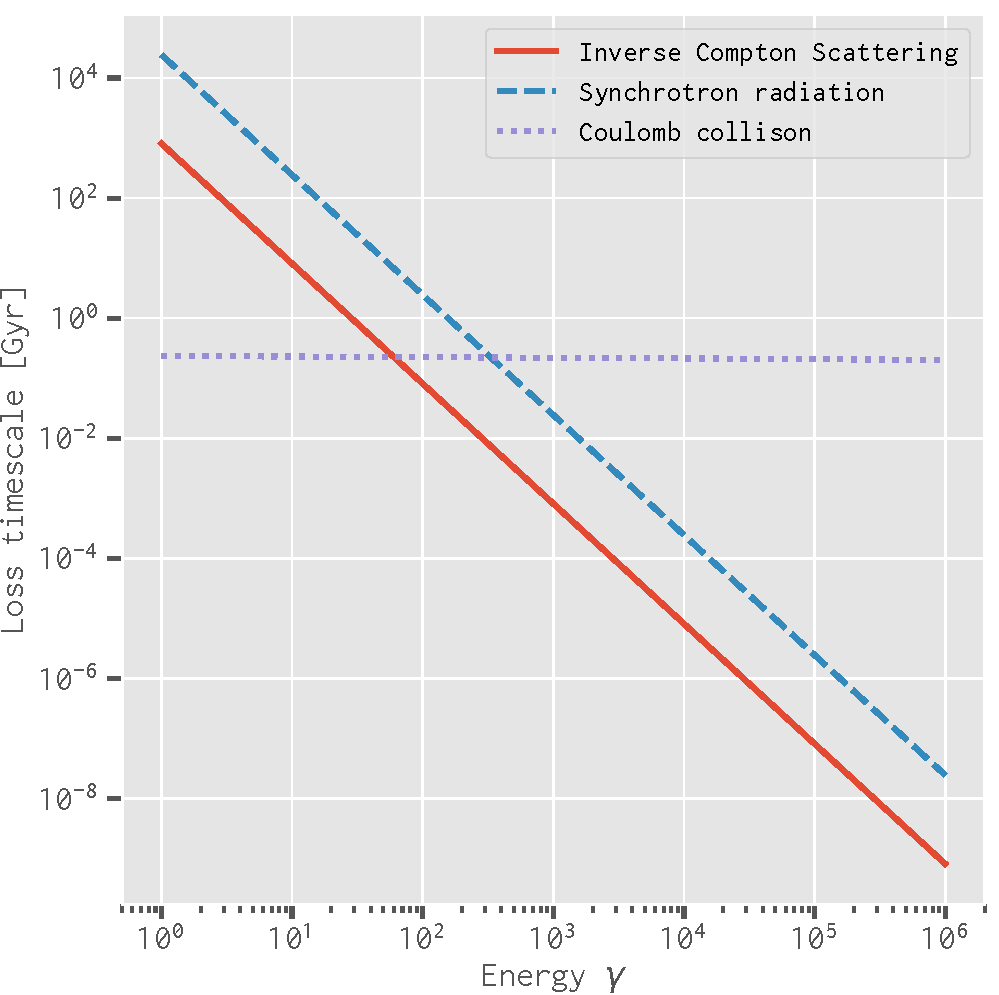
\includegraphics[width=0.7\textwidth]{energy-loss-timescale}
  \bicaption[电子的三种主要能量损失机制的时标对比]{%
    在 ICM 中,电子的三种主要能量损失机制的时标 $\tau_{\R{loss}}$ 对比,
    包括逆 Compton 散射(红色实线)、同步辐射(蓝色虚线)和 Coulomb 碰撞(紫色点线).
    使用的参数为:
    $\acs{n-th} = \SI{e-4}{\per\cubic\cm}$、
    $\acs{mag-field} = \SI{1}{\uG}$ 和 $z = 0.3$.
  }{%
    The comparison of timescale $\tau_{\R{loss}}$ among the three
    major energy loss mechanisms for electrons in the ICM,
    including the inverse Compton scattering (solid red line),
    synchrotron radiation (dashed blue line), and Coulomb collison
    (dotted purple line).
    The used parameters are:
    $\acs{n-th} = \SI{e-4}{\per\cubic\cm}$,
    $\acs{mag-field} = \SI{1}{\uG}$, and $z = 0.3$.
  }
  \label{fig:eloss-timescale}
\end{figure}

取 $\acs{n-th} = \SI{e-4}{\per\cubic\cm}$、
$\acs{mag-field} = \SI{1}{\uG}$ 和 $z = 0.3$ 为例,
\autoref{fig:eloss-timescale} 对比了这三种能量损失机制的\ac{timescale}
$\tau_{\R{loss}} = |\D{t}/\D{\ac{g}}|$.
可见,在高能端 ($\gamma \gtrsim 1000$),
逆 Compton 散射和\ac{rad-syn}是能量损失的主导机制;
在低能端 ($\gamma \lesssim 100$),
电子主要通过 Coulomb 碰撞而损失能量.
因此,中等能量 ($\gamma \sim 300$) 的电子具有很长的寿命 ($\sim$\,\SI{3}{\Gyr}),
能够随着\ac{gc}的成长而积累在 \ac{icm} 之中 \cite{sarazin1999}.

%---------------------------------------------------------------------
\subsection{数值实现}
\label{sec:numerical}

为了求解 Fokker--Planck 方程 [\autoref{eq:fokkerplanck}]
获得电子能谱随时间的演化,必须借助于数值算法.
本工作采用了由 \citeay{chang1970} 提出的\ac{finite-diff-scheme},
同时采用\ac{no-flux}边界条件 \cite{park1996}.
该算法的具体介绍可参见\autoref{app:fpsolver}.

在\ac{no-flux}边界条件下,电子可能在边界处出现不合理的堆积.
因此需要在两个边界处分别设置一个\enquote{缓冲区},
设其能量区间分别为:
$[\ac{g}_{\R{min}}, \ac{g}_{\R{buf1}}]$ 和
$[\ac{g}_{\R{buf2}}, \ac{g}_{\R{max}}]$.
在求解过程中,利用缓冲区外 ($\ac{g}_{\R{buf1}} < \ac{g} < \ac{g}_{\R{buf2}}$)
的有效能谱,按幂律形式外延并替换缓冲区内的能谱 \cite{borovsky1986,donnert2014}.
本文选取了 $\ac{g}_{\R{min}} = 1$ 和 $\ac{g}_{\R{max}} = \num{e6}$,
并采用对数网格 (grid) 将 \ac{g} 划分为 256 个单元 (cell),
其中两个缓冲区均占据 10 个单元.

求解 Fokker--Planck 方程还需要知道初始的电子能谱 $n_e(\ac{g}, t_0)$.
为此,首先假定 \ac{icm} 中积累的电子能谱为:
\begin{equation}
  \tilde{n}_e(\ac{g}) = Q_e(\ac{g}) \,\tau_0 ,
\end{equation}
其中 $\tau_0 \simeq t_{\R{merger}}^{(1)}$ 为星系团在第一次并合开始时刻的年龄.
然后在没有并合引起的湍流加速的情况下,
即\autoref{eq:energy-turb} 中的 $E_m \equiv 0$ 以及
$\ac{v-turb} \equiv \ac{v-turb0}$,
让电子能谱 $\tilde{n}_e(\ac{g})$ 演化 \SI{1}{\Gyr},
于是获得初始电子能谱 $n_e(\ac{g}, t_0)$ 的一个合理近似 \cite{brunetti2007}.

尽管一次并合的全部过程可能持续约 \SIrange{2}{3}{\Gyr} \cite{tormen2004,cassano2016},
但是在这个过程中,并合能够产生足够强的\ac{turbulence}以有效地加速电子的时间却比较短
($\lesssim$\,\SI{1}{\Gyr}).
这段有效加速时长 \ac{tau-turb} 可估算为 \cite{miniati2015}:
\begin{equation}
  \ac{tau-turb} \simeq \frac{2\,\ac{r-turb}}{\ac{v-imp}} .
\end{equation}

一个\ac{gc}在其过去的 $t_{\R{back}} = \SI{3}{\Gyr}$ 可能经历多次并合.
对于每一次并合
$\left( M^{(i)}_{\R{vir,m}}, M^{(i)}_{\R{vir,s}}, t^{(i)}_{\R{begin}} \right)$,
其中 $t^{(i)}_{\R{begin}} = t^{(i)}_{\R{merger}}$ 表示该并合的开始时间,
能够引起有效的流湍加速(即认为并合是活跃的)的时间段为
$\left[ t^{(i)}_{\R{begin}}, t^{(i)}_{\R{end}} \right]$,
其中 $t^{(i)}_{\R{end}} = t^{(i)}_{\R{begin}}+\tau^{(i)}_{\R{turb}}$
是此次并合变得不活跃的时间.
在其他没有并合活动的时间段里,则只有初始湍流对电子的加速有一定程度的贡献
[\autoref{eq:v-turb0}].
然而,初始湍流很弱,所以加速效率很低,不足以平衡\ac{rad-syn}和逆 Compton 散射的能量损失.

对于一个经历多次并合的\ac{gc},每次并合所产生的湍流区域大小 (\ac{r-turb}) 是不同的.
为了考虑这个变化,首先确定最大湍流区域的半径 \ac{R-turb},
然后在计算具有较小湍流区域 ($\ac{r-turb} < \ac{R-turb}$) 的并合的加速过程时,
将加速后的电子能谱相应地稀释到半径为 \ac{R-turb} 的球形区域里.
具体而言,对于一次有效加速时间段为
$\left[ t^{(i)}_{\R{begin}}, t^{(i)}_{\R{end}} \right]$、
湍流区域半径为 $r^{(i)}_{\R{turb}}$ 的并合,
将电子能谱被此次并合所加速的部分,即
$n_e^{\R{diff}}(\ac{g}) =
n_e\!\left(\ac{g}, t^{(i)}_{\R{end}}\right) -
n_e\!\left(\ac{g}, t^{(i)}_{\R{begin}}\right)$,
按如下体积比例稀释:
\begin{equation}
  \label{eq:ratio-v}
  R_{\R{vol}} = \left[ \frac{r^{(i)}_{\R{turb}}}{\ac{R-turb}} \right]^3 .
\end{equation}

一旦获得所需的电子能谱 $\ac{n-e}$,
在频率 $\nu$ 处的\acl{syn-em} (synchrotron emissivity) 为 \cite{rybicki1979}:
\begin{equation}
  \label{sec:jnu-sync}
  % unit: [erg/s/Hz/cm^3]
  \ac{syn-em}(\nu) =
    \frac{\sqrt{3} \,\ac{e}^3 \ac{mag-field}}{\ac{mass-e}\ac{speed-light}^2}
    \!\int_{\ac{g}_{\R{min}}}^{\ac{g}_{\R{max}}}
    \!\!\!\int_0^{\Cpi/2}
    \! \ac{syn-kernel}\!\left( \frac{\nu}{\ac{freq-crit}} \right)
    \ac{n-e} \sin^2 \!\theta \,\D{\theta} \,\D{\ac{g}} ,
\end{equation}
其中
\ac{speed-light} 是\acl{speed-light},\ac{e} 是\acl{e},
$\theta$ 是电子与磁场 \ac{mag-field} 之间的\ac{pitch-angle},
\ac{freq-crit} 是电子的\acl{freq-crit}:
\begin{equation}
  \ac{freq-crit} = \frac{3}{2} \ac{g}^2 \ac{freq-larmor} \sin\theta ,
\end{equation}
其中 \ac{freq-larmor} 是电子的 \acl{freq-larmor}:
\begin{equation}
  \ac{freq-larmor} =
    \frac{\ac{e}\ac{mag-field}}{2\Cpi \ac{mass-e}\ac{speed-light}} ,
\end{equation}
还有 $\ac{syn-kernel}(\cdot)$ 是\acl{syn-kernel} (kernel function):
\begin{equation}
  \ac{syn-kernel}(x) = x \int_x^{\infty} K_{5/3}(y) \,\D{y} ,
\end{equation}
其中 $K_{5/3}(\cdot)$ 是 5/3 阶修正 Bessel 函数.

\begin{figure}[htp]
  \centering
  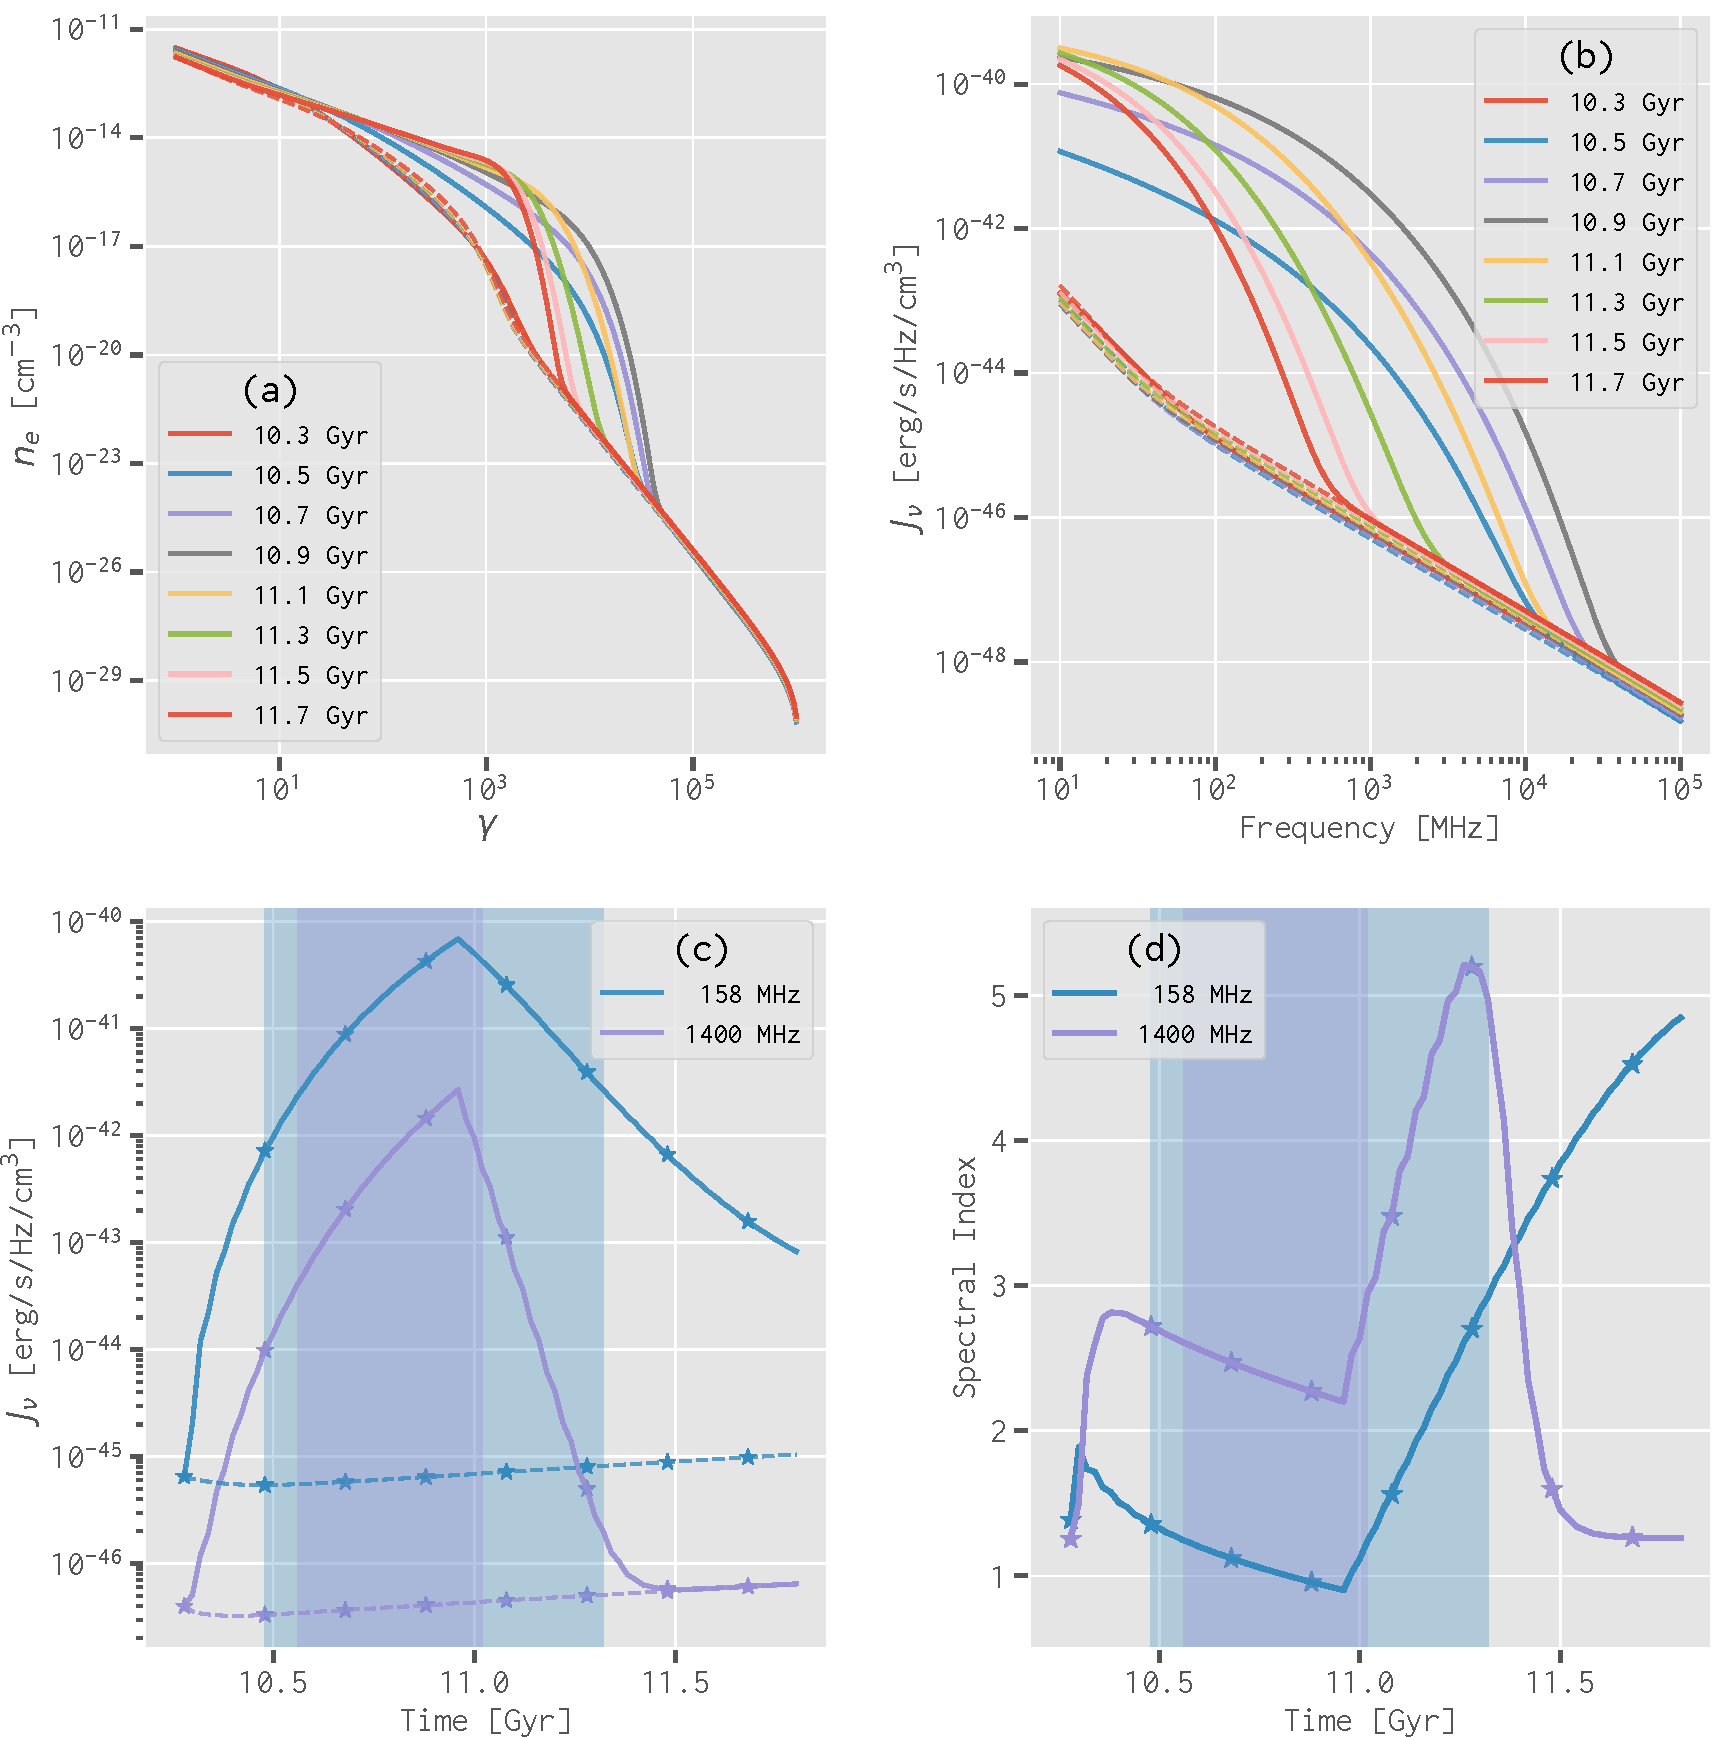
\includegraphics[width=0.98\textwidth]{spec-evo-example}
  \bicaption[电子能谱和同步辐射频谱随时间的演化示例]{%
    一个在红移 $z = 0.3$ ($t \simeq \SI{10.3}{\Gyr}$)
    经历了一次\acs*{m-major}的星系团从并合开始至
    $z = 0.15$ ($t \simeq \SI{11.8}{\Gyr}$)
    的高能电子能谱 \acs*{n-e} 和\acl*{syn-em}频谱
    $\acs*{syn-em}(\nu)$ 随时间的演化.
    \textbf{(a)}
    高能电子能谱(实线)和相应的参考能谱(虚线;见 \autoref{sec:halo-size});
    \textbf{(b)}
    \acl*{syn-em}频谱(实线)和相应的参考频谱(虚线);
    \textbf{(c)}
    同步辐射在 \SI{158}{\MHz} (蓝色实线)和 \SI{1400}{\MHz} (紫色实线)
    处的发射率及其相应的参考发射率(虚线)随时间的变化;
    \textbf{(d)}
    \SI{158}{\MHz} (蓝线)和 \SI{1400}{\MHz} (紫线)处的谱指数随时间的变化.
    阴影区域显示了射电晕存在的时间段(详见 \autoref{sec:halo-size}).
    星号标记了显示在子图 (a) 和 (b) 中的频谱所对应的时间点.
  }{%
    The temporal evolution of the electron and synchrotron
    emissivity spectra for an example cluster with one major merger,
    which begins at redshift $z = 0.3$ (i.e., $t \simeq \SI{10.3}{\Gyr}$)
    and is tracked until $z = 0.15$ (i.e., $t \simeq \SI{11.8}{\Gyr}$).
    \textbf{(a)} The relativistic electron spectra (solid lines) and the
    corresponding reference electron spectra (dashed lines; see
    \autoref{sec:halo-size}).
    \textbf{(b)} The synchrotron emissivity spectra (solid lines) and the
    corresponding reference synchrotron spectra (dashed lines).
    \textbf{(c)} The variation of \SI{158}{\MHz} (solid blue line) and
    \SI{1400}{\MHz} (solid purple line) synchrotron emissivity as well as
    the corresponding reference emissivity (dashed lines) with time.
    \textbf{(d)} The temporal variation of spectral indices at
    \SI{158}{\MHz} (blue line) and \SI{1400}{\MHz} (purple line).
    Shaded regions show the periods during which the radio halo exists
    (see \autoref{sec:halo-size}).
    Asterisks mark the time points corresponding to the spectra presented
    in panels (a) and (b).
  }
  \label{fig:spec-evo}
\end{figure}

以一个经历一次\ac{m-major}、质量为 \SI{e15}{\solarmass} 的星系团为例,
\autoref{fig:spec-evo} 显示了并合过程中高能电子能谱 \ac{n-e}
和\acl{syn-em}频谱 $\ac{syn-em}(\nu)$ 随时间的演化.
星系团在红移 $z = 0.3$ (对应宇宙年龄 $t \simeq \SI{10.3}{\Gyr}$)
时与一个质量为 \SI{6e14}{\solarmass} 的子团开始并合.
该并合的有效加速时长约为 $\tau_{\R{turb}} \simeq \SI{0.67}{\Gyr}$,
使电子被加速到极高能量 ($\gamma \gtrsim \num{e4}$),
形成在中高频段 ($> \si{\GHz}$) 可见的\ac{rh}.
然而,当并合变得不活跃时 ($t > \SI{10.9}{\Gyr}$),
高能端的电子迅速地损失能量而衰减,\ac{rh}也很快地消失,特别是在中高频段.

%---------------------------------------------------------------------
\subsection{识别和大小}
\label{sec:halo-size}

从上一节的示例可知,如果 \ac{icm} 中没有活跃的湍流加速,
\ac{rh}要么无法形成要么会迅速消失.
通过求解 Fokker--Planck 方程 [\autoref{eq:fokkerplanck}]
并得到对应\ac{gc}\enquote{当前}时刻的高能电子能谱 $n_e(\ac{g}, t_{\R{sim}})$ 后,
还需要判别\ac{rh}在频率 $\nu$ 处是否确实存在.
为此,本工作采用以下两点判据:
\begin{enumerate}
  \item \acl{syn-em}在频率 $\nu$ 的值 $\ac{syn-em}(\nu)$
    是相应的\enquote{参考值} $J'_{\R{syn}}(\nu)$ 的至少 1000 倍.
    该参考值 $J'_{\R{syn}}(\nu)$ 由相应的参考电子能谱
    $n'_e(\ac{g}, t_{\R{sim}})$ 确定,
    后者的计算方法与 \autoref{sec:numerical} 中计算初始电子能谱
    $n_e(\ac{g}, t_0)$ 的方法类似,
    即在没有并合引起的湍流加速的情况下求解 Fokker--Planck 方程而得到.

  \item 同步辐射在频率 $\nu$ 处谱指数满足 $\alpha_{\nu} \le 3$.
\end{enumerate}

对于\autoref{fig:spec-evo} 所示的例子,
\ac{rh}在 \SI{1.4}{\GHz} 处的存在时间段约为 \SIrange{10.6}{11.0}{\Gyr},
在 \SI{158}{\MHz} 处的存在时间段约为 \SIrange{10.5}{11.3}{\Gyr}.
同时,\ac{rh}的同步辐射频谱在 \SI{1.4}{\GHz} 和 \SI{158}{\MHz}
的谱指数分别达到了约 2.1 和 1.0.
这些结果显示,\ac{rh}在低频波段 ($\lesssim$\,\SI{200}{\MHz}) 更容易形成,
并且拥有更长的寿命.
因此,在低频波段也更容易发现更多的\ac{rh}.
此外,上述示例给出的 \SI{1.4}{\GHz} 谱指数 ($\alpha_{1400} \sim 2.1$)
比通常的观测结果\cite{feretti2012}偏大一些,
这是因为本文直接在一个频率 $\nu$ 附近计算该频率处的谱指数 $\alpha_{\nu}$,
而观测给出的谱指数 $\alpha_{\nu_1}^{\nu_2}$ 通常从两个相隔较远的频率
($\nu_1$ 和 $\nu_2$) 的观测数据得出,比如 0.3 和 1.4 GHz \cite{feretti2012}.

判别一个\ac{rh}存在后,接着需要确定其大小.
之前的研究已显示\acl{r-halo} \ac{r-halo}
会随\ac{gc}的\acl{r-vir} \ac{r-vir} 超线性地增大 \cite{cassano2007,basu2012},
这可能是由于高能电子和磁场的径向分布特征造成的 \cite{dolag2002}.
据此,我们假定\acl{r-halo} \ac{r-halo} 满足以下\ac{scaling-relation}:
\begin{equation}
  \label{eq:r-halo}
  \ac{r-halo} = f_r \ac{R-turb}
    \left( \frac{\ac{r-vir}}{r_{\R{vir,*}}} \right)^b ,
\end{equation}
其中
\ac{R-turb} 是最大湍流区域的半径 [另见\autoref{eq:ratio-v}],
$r_{\R{vir,*}}$ 是质量为 \SI{e15}{\solarmass} 的参考星系团的\acl{r-vir},
$f_r$ 和 $b$ 分别是\ac{scaling-relation}的系数和指数.
\citeay{cassano2007} 获得的观测\ac{scaling-relation}为:
$\ac{r-halo} \propto r_{\R{vir}}^{2.63 \pm 0.50}$,
与之对比后,我们选取 $f_r = 0.7$ 和 $b = 1.8$.

于是,\ac{rh}在频率 $\nu$ 处的功率 $\ac{P-halo}(\nu)$ 为:
\begin{equation}
  \label{eq:halo-power}
  \ac{P-halo}(\nu) = \frac{4\Cpi}{3} r_{\R{halo}}^3 \ac{syn-em}(\nu) ,
\end{equation}
同时在该频率处的流量密度 $\ac{S-halo}(\nu)$ 为:
\begin{equation}
  \label{eq:halo-flux}
  \ac{S-halo}(\nu) =
    \frac{(1+z_{\R{sim}}) \,\ac{P-halo}[\nu(1+z_{\R{sim}})]}{
      4\Cpi D_{\!L}^2(z_{\R{sim}})} ,
\end{equation}
其中
$\acs{D-luminosity}(z_{\R{sim}})$ 是\ac{rh}的\acl{D-luminosity},
因子 $(1 + z_{\R{sim}})$ 用于考虑 $K$ 修正 \cite{hogg1999}.

%---------------------------------------------------------------------
\subsection{模型参数和结果}
\label{sec:halo-results}

本工作对\ac{rh}构建的模型主要包含以下 5 个待调节的参数:
\begin{enumerate}
  \item \ac{f-injection}:
    注入电子的总能量密度与 \ac{icm} 热能密度 \ac{e-th} 之比;
  \item \ac{f-trans}:
    并合释放的能量中转化为湍流能量的比例;
  \item \ac{f-cr}:
    宇宙射线的能量密度与 \ac{icm} 热能密度 \ac{e-th} 之比;
  \item \ac{f-turb}:
    初始湍流的能量密度与 \ac{icm} 热能密度 \ac{e-th} 之比;
  \item \ac{f-instability}:
    \ac{icm} 等离子体的不稳定性参数.
\end{enumerate}
由于目前的观测和理论研究均无法给出上述参数的有效约束,
因此有必要仔细调节这些参数,使得模型给出的结果能够符合目前的观测结果,
主要包括\ac{f-flux}、射电晕的功率与宿主星系团的质量之间的\ac{scaling-relation}.

我们通过以下两个对比来调节上述参数.
第一个对比是射电晕的 \SI{1.4}{\GHz} 功率 ($P_{1400}$)
与宿主星系团的维里质量 (\ac{M-vir}) 之间的\ac{scaling-relation}.
观测的\ac{scaling-relation}由 \citeay{cassano2013} 给出:
$P_{1400} \propto M_{500}^{3.70 \pm 0.56}$.
这里需要将质量 $M_{500}$ 换算至维里质量以便与模拟结果对比,
具体换算方法可见附录 \autoref{sec:r-m-conv}.

另一个对比则利用 \SI{1.4}{\GHz} 全天积分的\ac{f-flux}.
为此,我们搜集了目前(截至 2018 年 1 月;TODO)已观测到的 80 个\ac{rh},
其中 71 个已确认,另外 9 个为候选,
详见\autoref{app:halos} 中的\autoref{tab:halos}.
考虑到目前观测到的\ac{rh}远不完备,尤其是在低流量端,
因此在对比时只要求模拟得到的\ac{f-flux}与观测结果在高流量端一致.

\begin{figure}[htp]
  \centering
  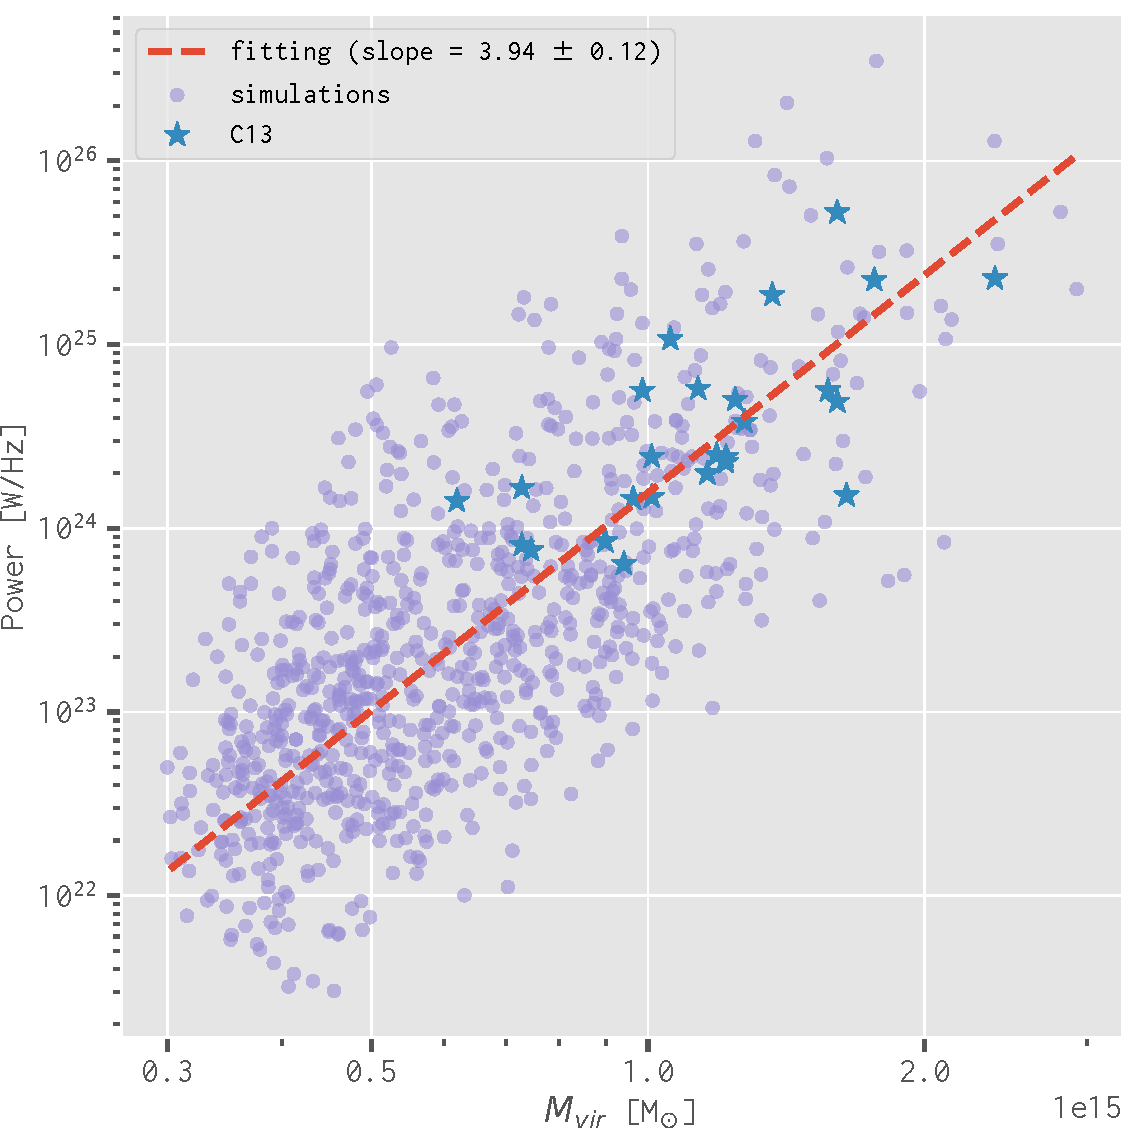
\includegraphics[width=0.7\textwidth]{halo-power-mvir}
  \bicaption[射电晕 \SI{1.4}{\GHz} 功率和宿主星系团质量之间的标度关系]{%
    模拟得到的射电晕 \SI{1.4}{\GHz} 功率 ($P_{1400}$) 和宿主星系团质量
    (\acs*{M-vir}) 之间的标度关系.
    蓝色星号表示来自 \citeay{cassano2013} 的观测数据.
    紫色圆点表示 500 次模拟的结果,红色虚线为模拟结果的拟合线:
    $P_{1400} \propto M_{\R{vir}}^{3.94 \pm 0.12}$.
  }{%
    Simulated scaling relation between the radio halo power at
    \SI{1.4}{\GHz} ($P_{1400}$) and the cluster mass (\acs*{M-vir}).
    Blue asterisks mark the observation data from \citeay{cassano2013}.
    Purple dots represent the results of 500 simulation runs
    and the dashed red line shows the fitted relation of
    $P_{1400} \propto M_{\R{vir}}^{3.94 \pm 0.12}$.
  }
  \label{fig:halo-power}
\end{figure}

\begin{figure}[htp]
  \centering
  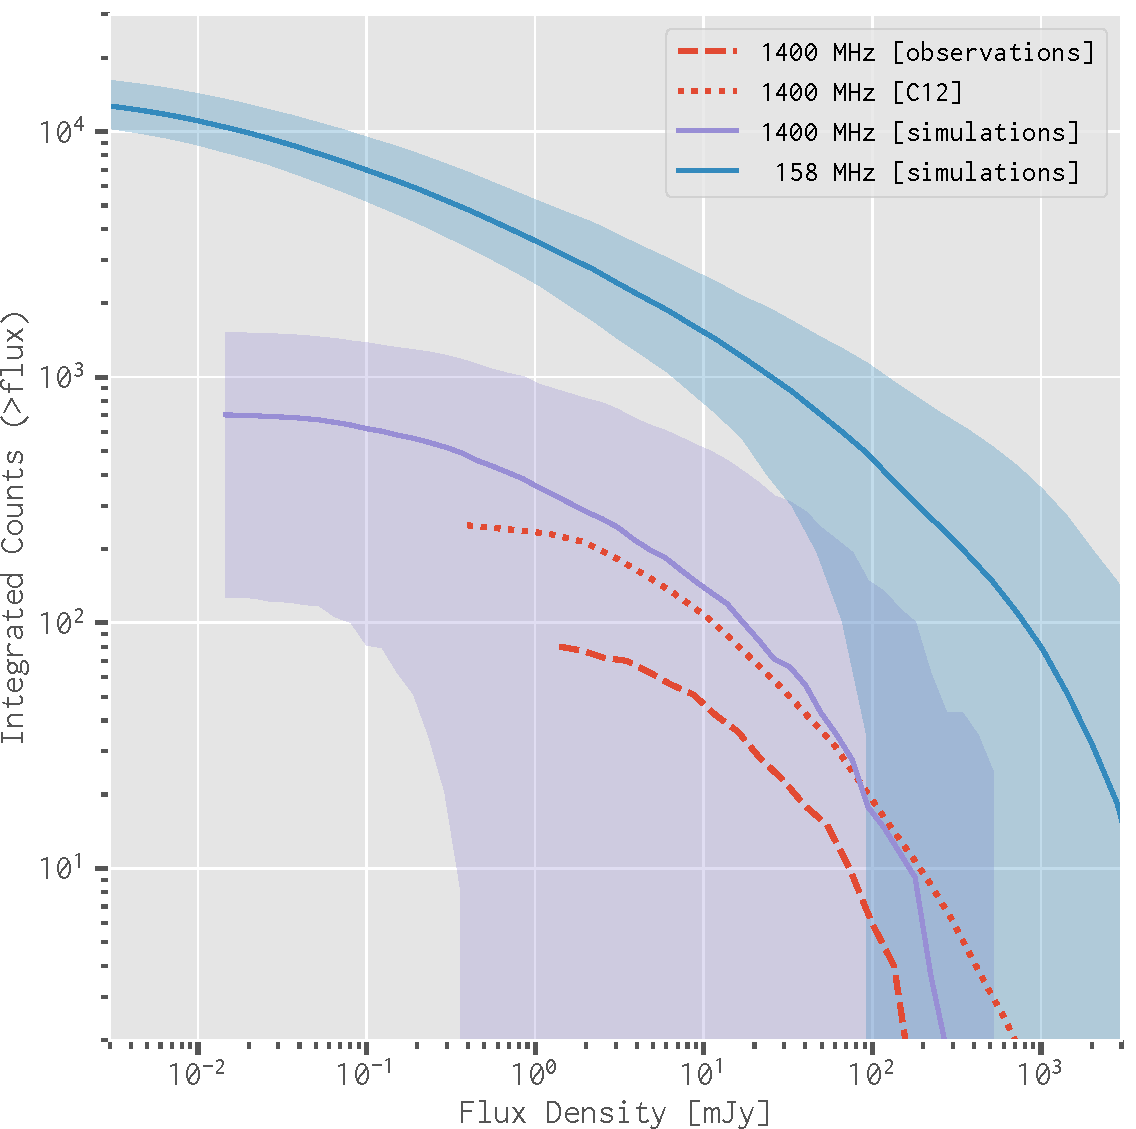
\includegraphics[width=\textwidth]{fluxfunc-simucomp}
  \bicaption[射电晕 \SI{1.4}{\GHz} 流量函数的对比]{%
    模拟的射电晕(紫色实线)和观测的射电晕(红色虚线)之间的
    \SI{1.4}{\GHz} 流量函数对比.
    红色点线显示了 \citeay{cassano2012} 预测的 \SI{1.4}{\GHz} 流量函数.
    作为对比,蓝色实线表示模拟的射电晕的 \SI{158}{\MHz} 流量函数.
    阴影区域显示了从 500 次模拟估算得到的 68\% 误差范围.
  }{%
    The \SI{1.4}{\GHz} all-sky integrated flux function comparison
    between the simulated (solid purple line) and observed
    (dashed red line) radio halos.
    The dotted red line shows the \SI{1.4}{\GHz} flux function
    predicted by \citeay{cassano2012}.
    The solid blue line represents the \SI{158}{\MHz} flux function for
    the simulated halos as a comparison.
    Shaded regions mark the 68\% uncertainties of the
    simulated radio halos estimated from the 500 simulation runs.
  }
  \label{fig:halos-simucomp}
\end{figure}

根据上述 $P_{1400}$--\ac{M-vir} \ac{scaling-relation}可知,
亮射电晕主要位于大质量 ($\gtrsim$\,\SI{e15}{\solarmass}) 星系团中.
在一片 \SI{10 x 10}{\degree} 的天区里,
大质量星系团有显著的涨落 (\autoref{sec:mass-function}),
因此亮射电晕也会出现明显的涨落.
为了考虑这个分布涨落,我们对每一种参数组合均重复模拟 500 次,
由此估算模拟结果的均值和误差,并与上述两点观测结果进行对比.
通过测试多种参数组合,最终选取如下一组参数:
$\ac{f-injection} = 0.01\%$、
$\ac{f-trans} = 15\%$、
$\ac{f-cr} = 1.5\%$、
$\ac{f-turb} = 1.5\%$ 以及
$\ac{f-instability} = 0.1$.

如\autoref{fig:halo-power} 所示,使用上述调节好的参数,
模拟的射电晕给出的 $P_{1400}$--\ac{M-vir} \ac{scaling-relation}为:
$P_{1400} \propto M_{\R{vir}}^{3.94 \pm 0.12}$.
该\ac{scaling-relation}的斜率和截距与 \citeay{cassano2013}
获得的观测结果都符合得很好.
\autoref{fig:halos-simucomp} 显示了 \SI{1.4}{\GHz} \ac{f-flux}
的对比结果,可见模拟的射电晕与观测的射电晕在高流量端是一致的.
同时,本工作模拟给出的 \SI{1.4}{\GHz} \ac{f-flux}
还与 \citeay{cassano2012} 的预测结果是匹配的.

此外,\autoref{fig:halo-fraction} 显示了具有射电晕的星系团比例
随星系团质量的变化.
显然,星系团的质量越大,其中存在射电晕的概率就越高.
同时,星系团中存在一个在低频波段(如 \SI{158}{\MHz})可见的射电晕的概率
也显著高于存在一个在高频波段(如 \SI{1.4}{\GHz})可见的射电晕.
因此,在低频波段 ($\sim$\,\SIrange{100}{200}{\MHz}) 将能观测到
成千上万个射电晕,远远多于目前发现的数目 \cite{cassano2012,cassano2015}.

\begin{figure}[htp]
  \centering
  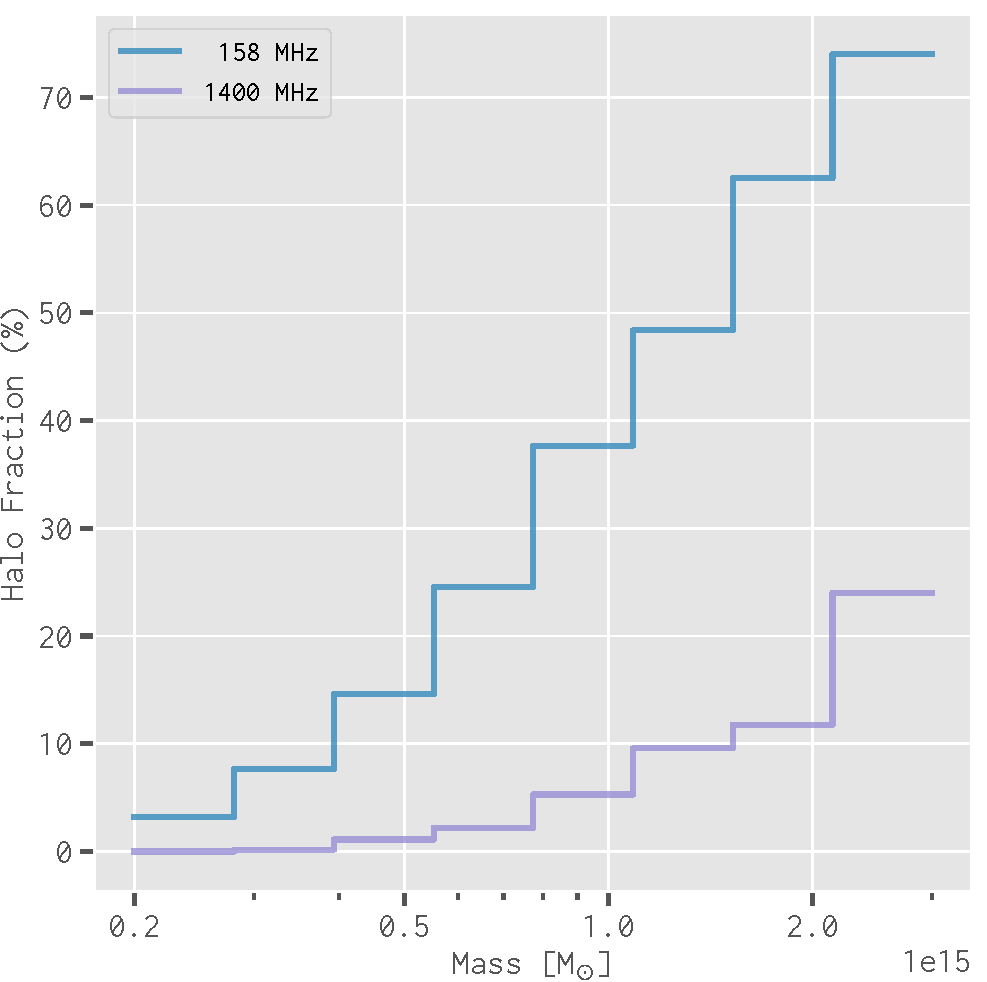
\includegraphics[width=0.7\textwidth]{halo-fraction}
  \bicaption[具有射电晕的星系团比例随星系团质量的变化]{%
    具有射电晕的星系团比例随星系团质量的变化.
    蓝线和紫线分别表示在 \SI{158}{\MHz} 和 \SI{1.4}{\GHz}
    频率处识别的射电晕比例.
  }{%
    The fraction of clusters with radio halos as a function of the cluster
    mass.
    The blue and purple lines represent the fraction of halos identified at
    \SI{158}{\MHz} and \SI{1.4}{\GHz}, respectively.
  }
  \label{fig:halo-fraction}
\end{figure}

%---------------------------------------------------------------------
\subsection{图像生成}
\label{sec:halo-maps}

获得射电晕的半径 \ac{r-halo} [\autoref{eq:r-halo}]
和流量密度 $\ac{S-halo}(\nu)$ [\autoref{eq:halo-flux}] 后,
为了生成图像,我们假定射电晕是圆形的,
并采用以下指数型轮廓来描述其角向平均的亮度分布 \cite{murgia2009}:
\begin{equation}
  \label{eq:halo-profile}
  \ac{I-nu}(\theta) =
    I_{\nu,0} \exp\left( -\frac{3\,\theta}{\theta_{\R{halo}}} \right) ,
\end{equation}
其中
$\theta = r / \acs{D-angular}(z_{\R{sim}})$ 是距离射电晕中心的角半径
(angular radius),
并且 $\ac{D-angular}(z_{\R{sim}})$ 是射电晕的\acl{D-angular};
$\theta_{\R{halo}} = \ac{r-halo} / \acs{D-angular}(z_{\R{sim}})$.
$I_{\nu,0}$ 为中心亮度,由射电晕的流量密度 $\ac{S-halo}(\nu)$ 确定:
\begin{align}
  \ac{S-halo}(\nu)
    & = \int_0^{\theta_{\R{halo}}} \ac{I-nu}(\theta) \,\D{\theta} \\
    & = I_{\nu,0} \int_0^{\theta_{\R{halo}}}
        \exp( -3\,\theta / \theta_{\R{halo}} ) \,\D{\theta} ,
\end{align}
于是可得:
\begin{equation}
  I_{\nu,0} = \frac{9 \ac{S-halo}(\nu)}{2\Cpi \theta^2_{\R{halo}}} .
\end{equation}
最后利用 Rayleigh--Jeans 近似 [\autoref{eq:rj-approx}],
便可以得到\ac{rh}的亮温度 $\acs{T-b}(\nu)$ 的分布图像.

如 \autoref{sec:halo-results} 所述,
为了考虑亮射电晕数目的显著涨落,使得\autoref{chap:halo}的评估结果更具代表性,
我们针对射电的模拟重复了 100 次,并将全部 100 次的模拟数据用于后续分析.
基于这 100 次模拟,射电晕的亮温度的\ac{rms}值的中位数以及 68\% 的误差\footnote{%
  68\% 的误差根据第 16 和第 84 \ac{percentile}得到.
  对于弥散很大的数据,如此计算的误差比标准差更稳健.
}为:
在 \SI{124}{\MHz} 处是
$\left(4.21_{-2.60}^{+11.2}\right) \times 10^3$ \si{\mK};
在 \SI{158}{\MHz} 处是
$\left(1.81_{-1.13}^{+5.28}\right) \times 10^3$ \si{\mK};
以及在 \SI{196}{\MHz} 处是
$\left(0.85_{-0.54}^{+2.74}\right) \times 10^3$ \si{\mK}
(另见\autoref{tab:tb-rms}).
\autoref{fig:halos-skymap} 显示了其中一次典型情况的
射电晕在 \SI{158}{\MHz} 的模拟天图.

\begin{figure}[htp]
  \centering
  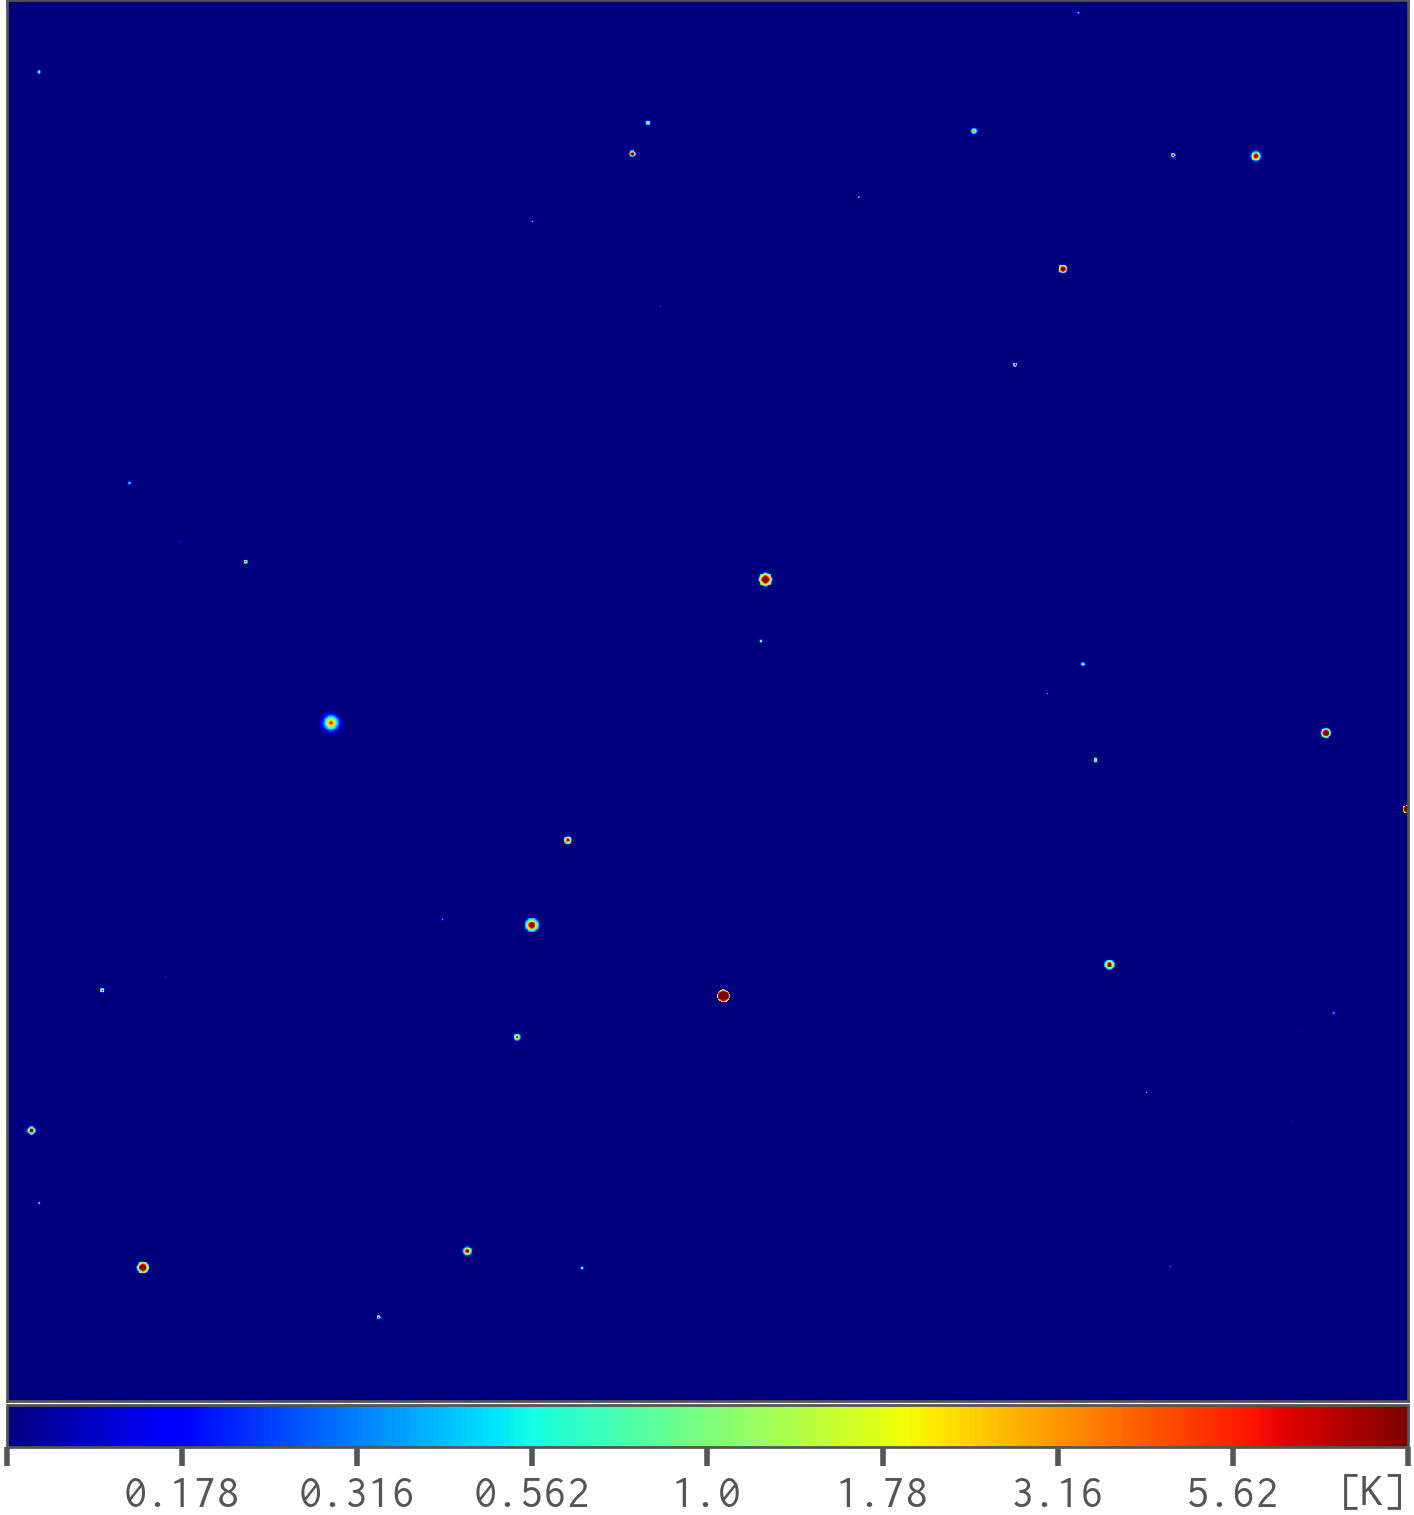
\includegraphics[width=0.8\textwidth]{skymap-halos-f158}
  \bicaption[射电晕在 \SI{158}{\MHz} 的模拟天图示例]{%
    射电晕在 \SI{158}{\MHz} 的模拟天图示例,为 100 次模拟中的一次典型情况.
    天区的大小为 \SI{10 x 10}{\degree},
    \ac{colorbar}以 \si{\kelvin} 为单位.
  }{%
    An typical example from the 100 simulation runs showing the
    simulated radio halos at \SI{158}{\MHz}.
    The sky region size is \SI{10 x 10}{\degree},
    and the color bar is in units of \si{\kelvin}.
  }
  \label{fig:halos-skymap}
\end{figure}

\begin{table}[htp]
  \centering
  \bicaption[所有成分的亮温度的\acs*{rms}值]{%
    所有成分在三个频带的中心频率处的亮温度的\acs*{rms}值(单位: mK)
  }{%
    The Root-Mean-Square Brightness Temperatures of All Components
    (unit: mK)
  }
  \label{tab:tb-rms}

  \begin{tabular}{cccc}
    \toprule
    成分 & \SI{124}{\MHz} & \SI{158}{\MHz} & \SI{196}{\MHz} \\
    \midrule
    射电晕(100 次模拟) &
      $\left(4.21_{-2.60}^{+11.2}\right) \times 10^3$ &
      $\left(1.81_{-1.13}^{+5.28}\right) \times 10^3$ &
      $\left(0.85_{-0.54}^{+2.74}\right) \times 10^3$ \\
    银河系同步辐射 & \num{4.74e5} & \num{2.52e5} & \num{1.43e5} \\
    银河系自由--自由辐射 & \num{330} & \num{200} & \num{130} \\
    河外点源 & \num{29.7e7} & \num{5.90e7} & \num{1.39e7} \\
    EoR 信号 & \num{15.1} & \num{11.3} & \num{3.77} \\
    \bottomrule
  \end{tabular}
\end{table}


%=====================================================================
\section{银河系}
\label{sec:simu-galactic}

在低频波段,银河系的弥散辐射主要包括\ac{rad-syn}和\ac{rad-ff}.
本节将介绍如何模拟这两种辐射成分的图像.

银河系的辐射随天空位置而发生显著变化,越靠近银盘辐射越强,
因此 EoR 实验将挑选高银纬天区开展观测.
考虑到 SKA1-Low 将建设在 \ac{mwa} (\ang{26;42;12}\,S, \ang{116;40;16}\,E)
的旁边,同时 \ac{mwa} 目前正在研究的一块 EoR 天区位于
(R.A., Dec.\@) = (\SI{0}{\degree}, \SI{-27}{\degree}) \cite{beardsley2016},
该天区位于高银纬 ($b = \SI{-78.5}{\degree}$) 区域,
而且几乎经过望远镜的\ac{zenith},是一个理想的观测天区.
这个天区对本工作所开展的模拟研究而言是一个合适的选择(另见 \autoref{sec:obs-simu}).
因此,我们将以 (R.A., Dec.\@) = (\SI{0}{\degree}, \SI{-27}{\degree})
为中心坐标模拟银河系弥散辐射的天图.

%---------------------------------------------------------------------
\subsection{同步辐射}

银河系\ac{rad-syn}在低频波段的天图通过以
Haslam \SI{408}{\MHz} 巡天图\cite{haslam1982}
为模板按幂律形式外延得到 \cite{wang2010,bonaldi2015}:
\begin{equation}
  T_b^{\R{syn}}(\B{\hat{r}}, \nu)
    = T_b^{\R{haslam}}(\B{\hat{r}}) \left( \frac{\nu}{\SI{408}{\MHz}}
      \right)^{-\alpha_{\R{syn}}(\B{\hat{r}})} ,
\end{equation}
其中 $T_b^{\R{haslam}}(\B{\hat{r}})$ 为银河系 $\B{\hat{r}}$ 处的
\SI{408}{\MHz} 亮温度,
$\alpha_{\R{syn}}(\B{\hat{r}})$ 为该处的同步辐射谱指数.

本工作使用了由 \citeay{remazeilles2015} 重新处理的 Haslam \SI{408}{\MHz}
全天图\footnote{%
  重新处理的 Haslam \SI{408}{\MHz} 全天图:
  \url{http://www.jb.man.ac.uk/research/cosmos/haslam_map/}}.
与 Haslam 原图相比,新图具有更好的仪器校准以及更准确的河外点源扣除 \cite{remazeilles2015}.
同步辐射的谱指数会随天空位置变化,
\citeay{giardino2002} 综合了 Haslam \SI{408}{\MHz} 全天图、
\SI{1420}{\MHz} 北天图 \cite{reich1986}
以及 \SI{2326}{\MHz} 南天图 \cite{jonas1998},
处理得到了的银河系同步辐射的谱指数全天分布图.
本工作利用了该谱指数分布图确定上式中的 $\alpha_{\R{syn}}(\B{\hat{r}})$.
\autoref{fig:galactic-skymaps} 左栏显示了银河系\ac{rad-syn}在
\SI{158}{\MHz} 的天图.
\autoref{tab:tb-rms} 中列出了在三个频带的中心频率处的亮温度的\ac{rms}值.

\begin{figure}[htp]
  \centering
  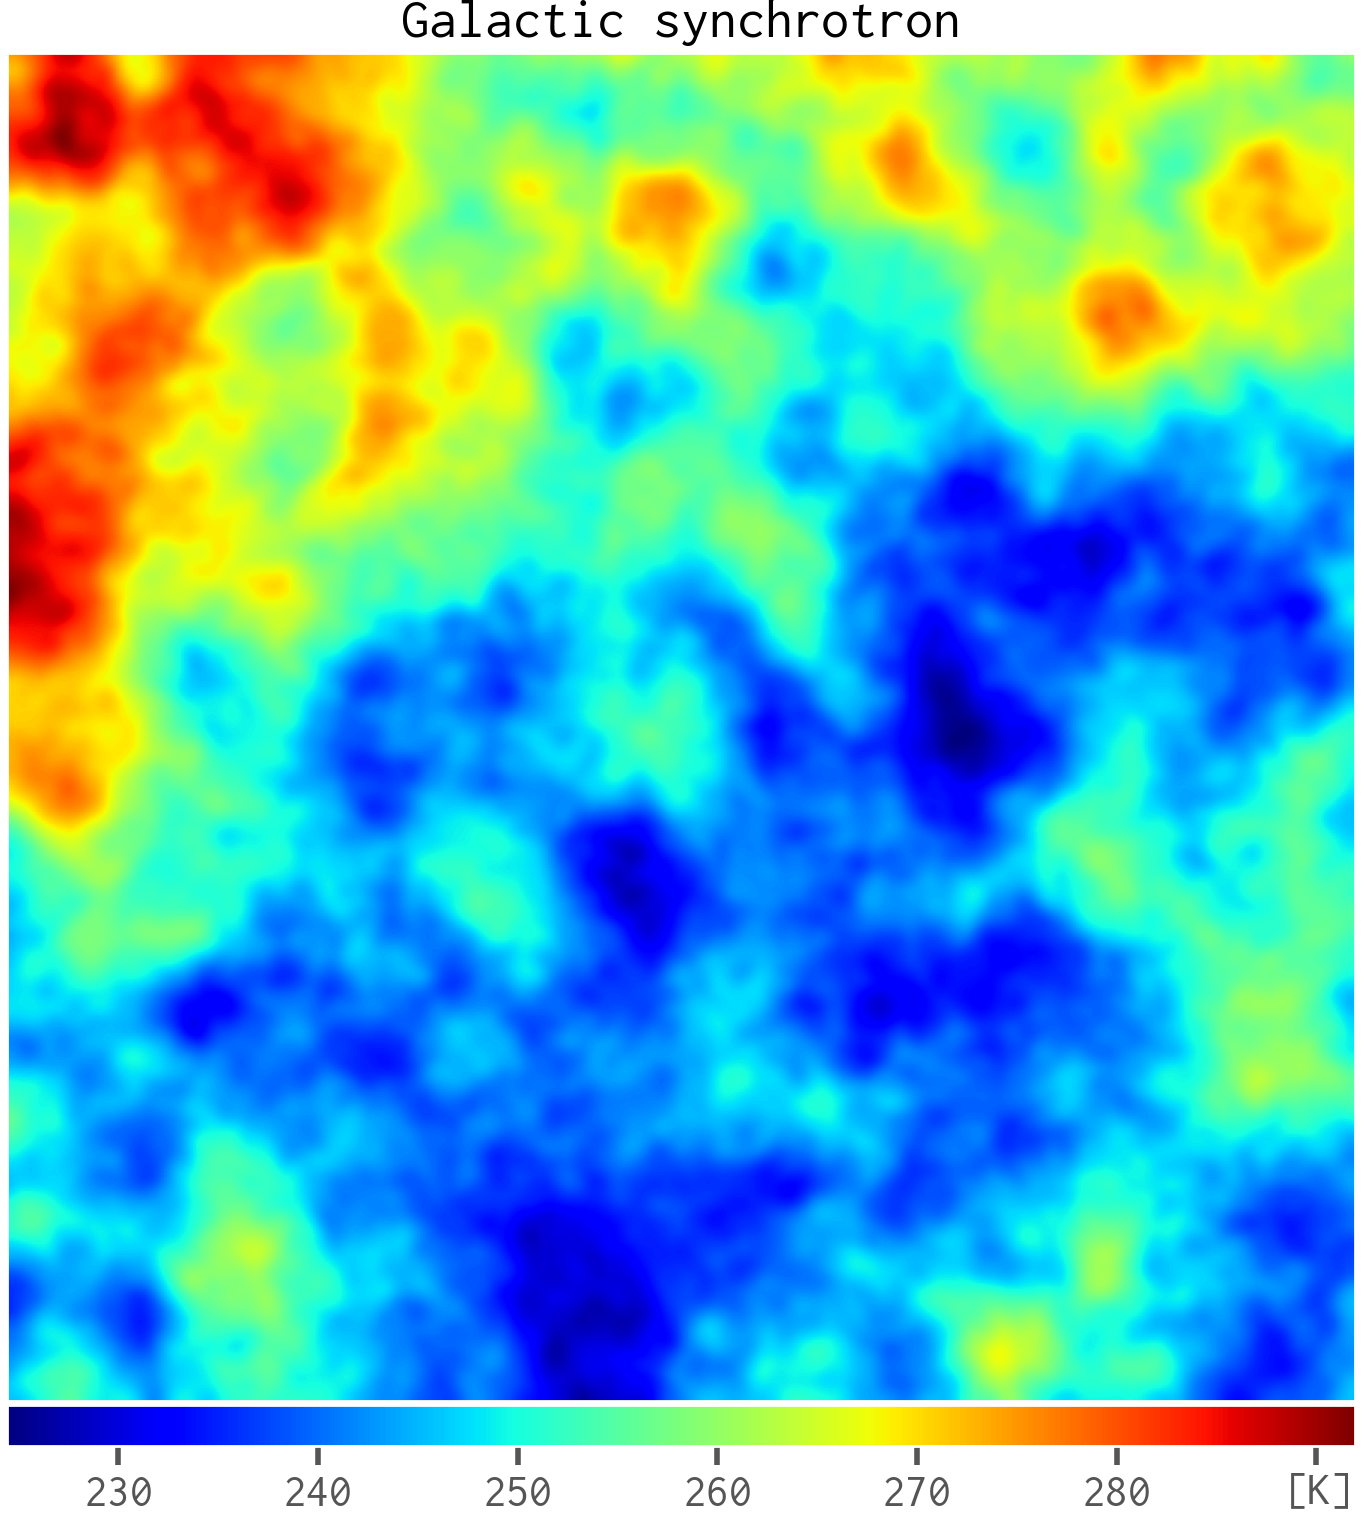
\includegraphics[width=0.498\textwidth]{skymap-gsyn-f158}%
  \hfill
  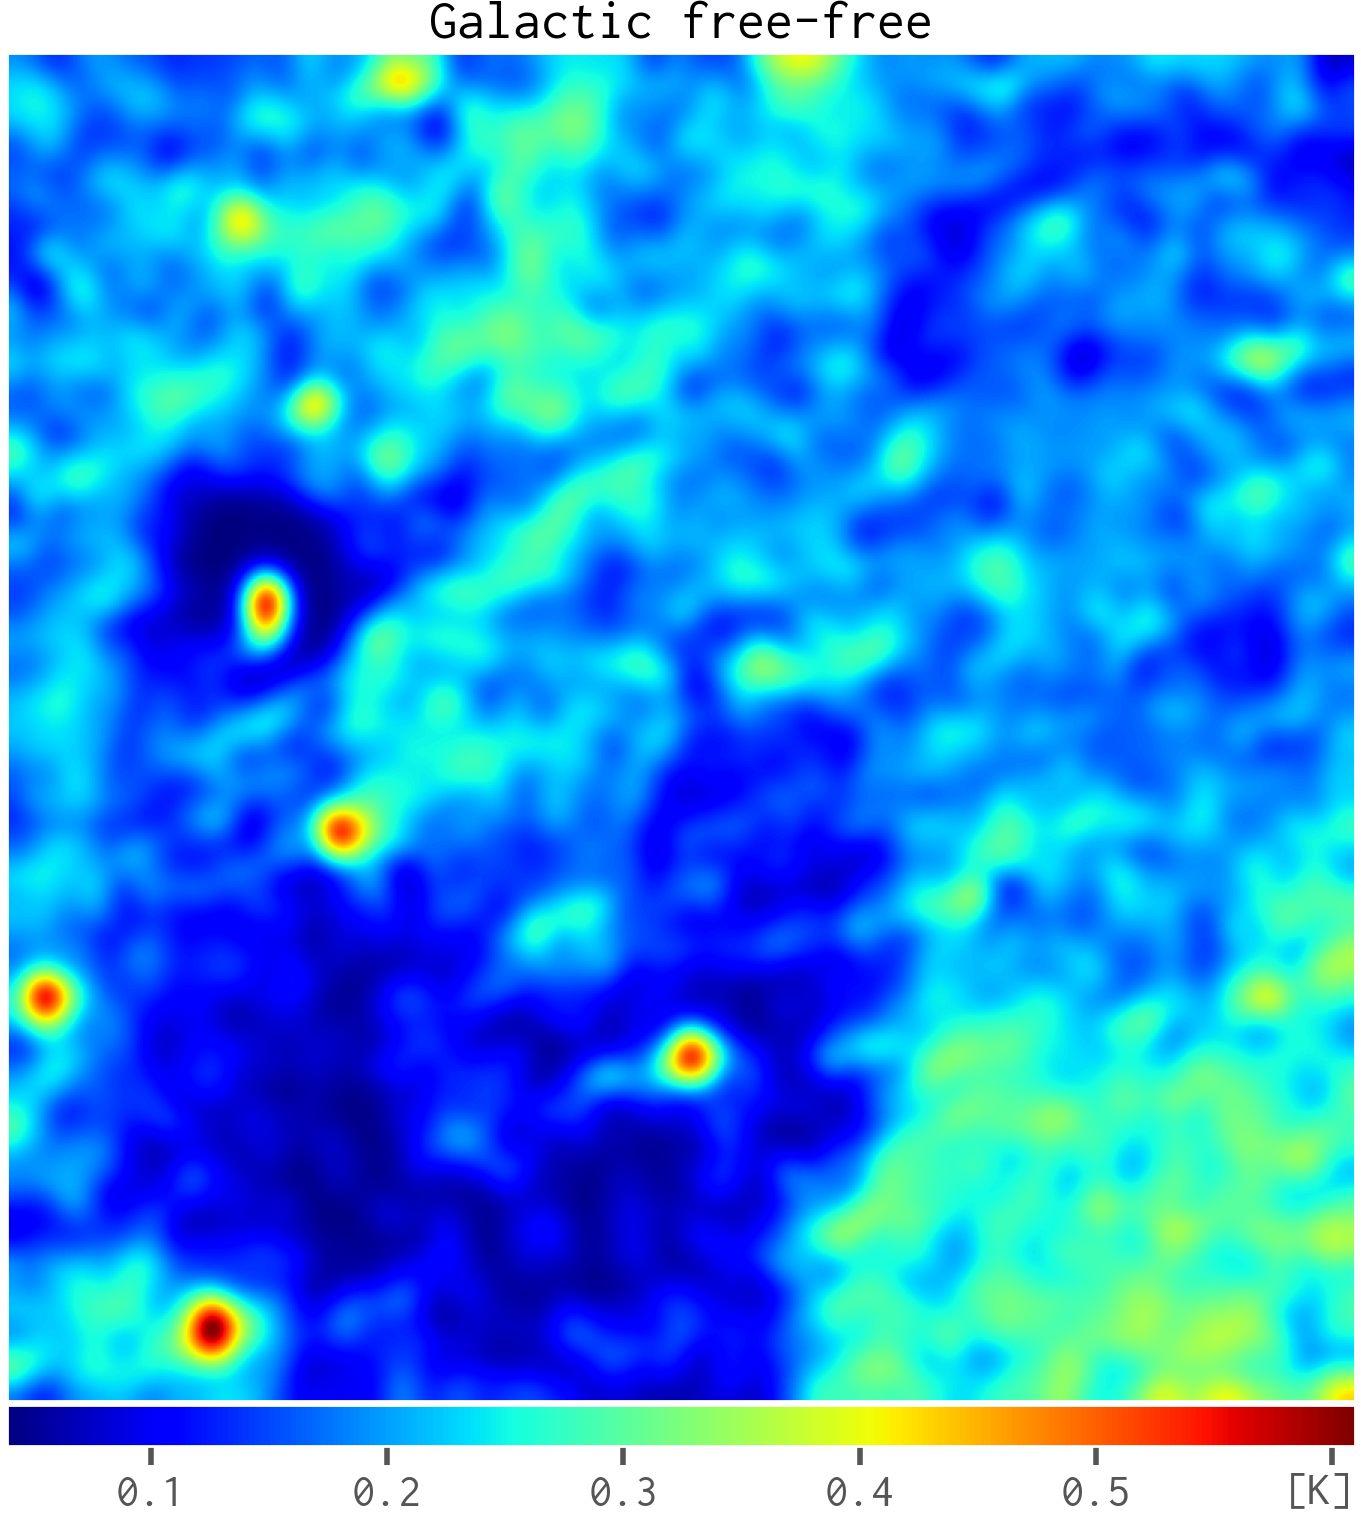
\includegraphics[width=0.498\textwidth]{skymap-gff-f158}
  \bicaption[银河系同步辐射和自由--自由辐射在 \SI{158}{\MHz} 的天图]{%
    银河系同步辐射(左栏)和自由--自由辐射(右栏)在 \SI{158}{\MHz} 的天图.
    天区的大小为 \SI{10 x 10}{\degree},
    \ac{colorbar}以 \si{\kelvin} 为单位.
  }{%
    The sky maps of the Galactic synchrotron (left panel)
    and free-free (right panel) radiations at \SI{158}{\MHz}.
    Both maps have a sky region size of \SI{10 x 10}{\degree}
    and the color bars are in units of \si{\K}.
  }
  \label{fig:galactic-skymaps}
\end{figure}

%---------------------------------------------------------------------
\subsection{自由--自由辐射}
\label{sec:simu-gff}

银河系\ac{rad-ff}和 Hα 源自相同的辐射区域(如\ac{hii}区、\ac{wim}),
因此两者之间存在紧密的联系 \cite{dickinson2003},
利用该关系以及 Hα 巡天图 \cite{finkbeiner2003},
便可以获得所需的银河系\ac{rad-ff}的图像.

由于 Hα 辐射易被尘埃吸收,而\ac{rad-ff}则几乎不受尘埃的影响,
所以首先需要对观测到的 Hα 辐射 $I_{\R{Hα}}(\B{\hat{r}})$
修正尘埃吸收 \cite{dickinson2003}:
\begin{equation}
  I_{\R{Hα}}^{\R{corr}}(\B{\hat{r}})
    = I_{\R{Hα}}(\B{\hat{r}}) \times 10^{0.0185 f_d D(\B{\hat{r}})} ,
\end{equation}
其中
$D(\B{\hat{r}})$ 是视线方向 $\B{\hat{r}}$ 上的尘埃\ac{column-density},
以 [\si{\mega\jansky\per\steradian}] 为单位,
$f_d$ 是尘埃在视线方向上的有效吸收比例.
接着,\ac{rad-ff}在频率 $\nu$ 处的图像 $T_b^{\R{ff}}(\B{\hat{r}}, \nu)$
可由以下关系计算得到 \cite{dickinson2003}\footnote{%
  \citeay{dickinson2003} 的公式 (11) 中的 \enquote{$\times\num{e3}$} 是多余的.
}:
\begin{equation}
  T_b^{\R{ff}}(\B{\hat{r}}, \nu)
    = 38.86 \,\nu^{-2.1} 10^{(290/T_e)} \, T_e^{0.667} \,a(\nu, T_e)
      \left[ \frac{I_{\R{Hα}}^{\R{corr}}(\B{\hat{r}})}{\si{\rayleigh}}
      \right] \quad [\si{\kelvin}] ,
\end{equation}
其中
$T_e$ 是辐射区域的电子温度(以 \si{\kelvin} 为单位),
频率 $\nu$ 的单位是 \si{\MHz},
因子 $a(\nu, T_e)$ 是对\acl{optical-depth}的修正,由下式给出:
\begin{equation}
  a(\nu, T_e) =
    0.183 \,\nu^{0.1} T_e^{-0.15}
    \left[ 3.91 - \ln \nu + 1.5 \ln T_e \right] .
\end{equation}

与 \citeay{dickinson2003} 一致,本工作采用 $f_d = 0.33$
和 $T_e = \SI{7000}{\kelvin}$.
再利用 \citeay{finkbeiner2003} 提供的 Hα 辐射全天图
以及来自 \citeay{schlegel1998} 的全天尘埃分布图,
便可获得银河系\ac{rad-ff}在低频波段的天图.
\autoref{fig:galactic-skymaps} 右栏显示了银河系\ac{rad-ff}在 \SI{158}{\MHz} 的天图.
\autoref{tab:tb-rms} 中列出了该前景成分在三个频带的中心频率处的亮温度的\ac{rms}值.


%=====================================================================
\section{河外点源}
\label{sec:simu-eg-point}

\begin{figure}[htp]
  \centering
  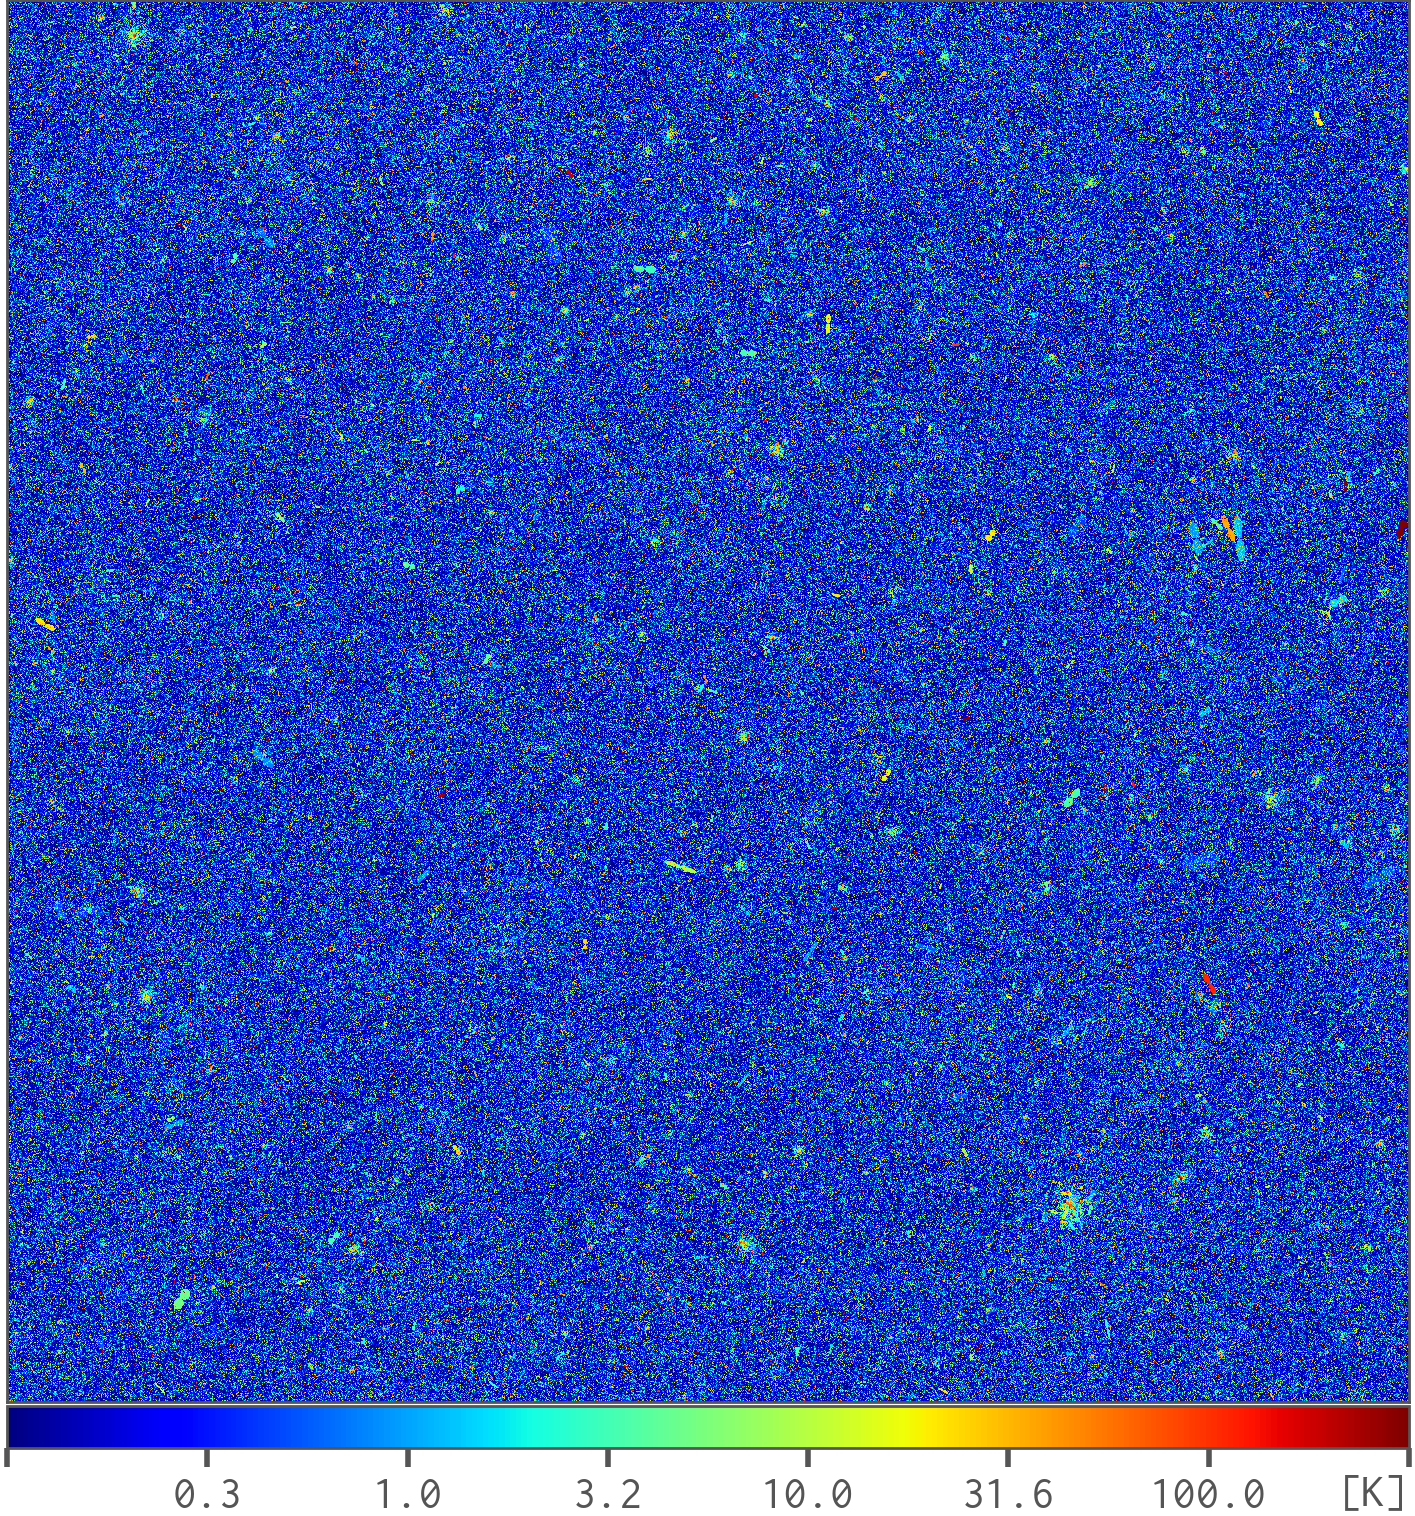
\includegraphics[width=0.7\textwidth]{skymap-ptrsrc-f158}
  \bicaption[河外点源在 \SI{158}{\MHz} 的模拟天图]{%
    河外点源在 \SI{158}{\MHz} 的模拟天图.
    天区的大小为 \SI{10 x 10}{\degree},
    \ac{colorbar}以 \si{\kelvin} 为单位.
  }{%
    The simulated sky map of the extragalactic point sources at \SI{158}{\MHz}.
    The sky region size is \SI{10 x 10}{\degree}
    and the color bar is in units of \si{\K}.
  }
  \label{fig:ptrsrc-skymap}
\end{figure}

本工作对河外点源的模拟继承自我们之前的一项工作\cite{wang2010},
其中模拟了以下几类点源 \cite{snellen2000,wilman2008,wang2010}:
\begin{enumerate}
  \item 恒星形成星系,
    包括普通晚型星系 (normal late-type galaxy) 和星暴星系 (starburst galaxy);
  \item 射电宁静 (radio-quiet) \ac{agn};
  \item \ac{fr} I 型和 II 型 \ac{agn};
  \item GHz 倒转谱和致密陡谱射电星系.
\end{enumerate}
上述第 1--3 类点源的模拟使用了 \citeay{wilman2008} 针对 SKA 模拟的点源结果;
第 4 类点源的模拟则利用了相应的\ac{f-luminosity}和频谱模型
\cite{oDea1998,snellen1998,fanti2001}.
具体模拟方法可参考 \citeay{wang2010} 和 \citeay{wilman2008} 及其所引文献.
\autoref{fig:ptrsrc-skymap} 显示了模拟的河外点源在 \SI{158}{\MHz} 的天图.
在三个频带的中心频率处的亮温度的\ac{rms}值罗列在\autoref{tab:tb-rms} 中.


%=====================================================================
\section{EoR 信号}
\label{sec:simu-eor}

\begin{figure}[htp]
  \centering
  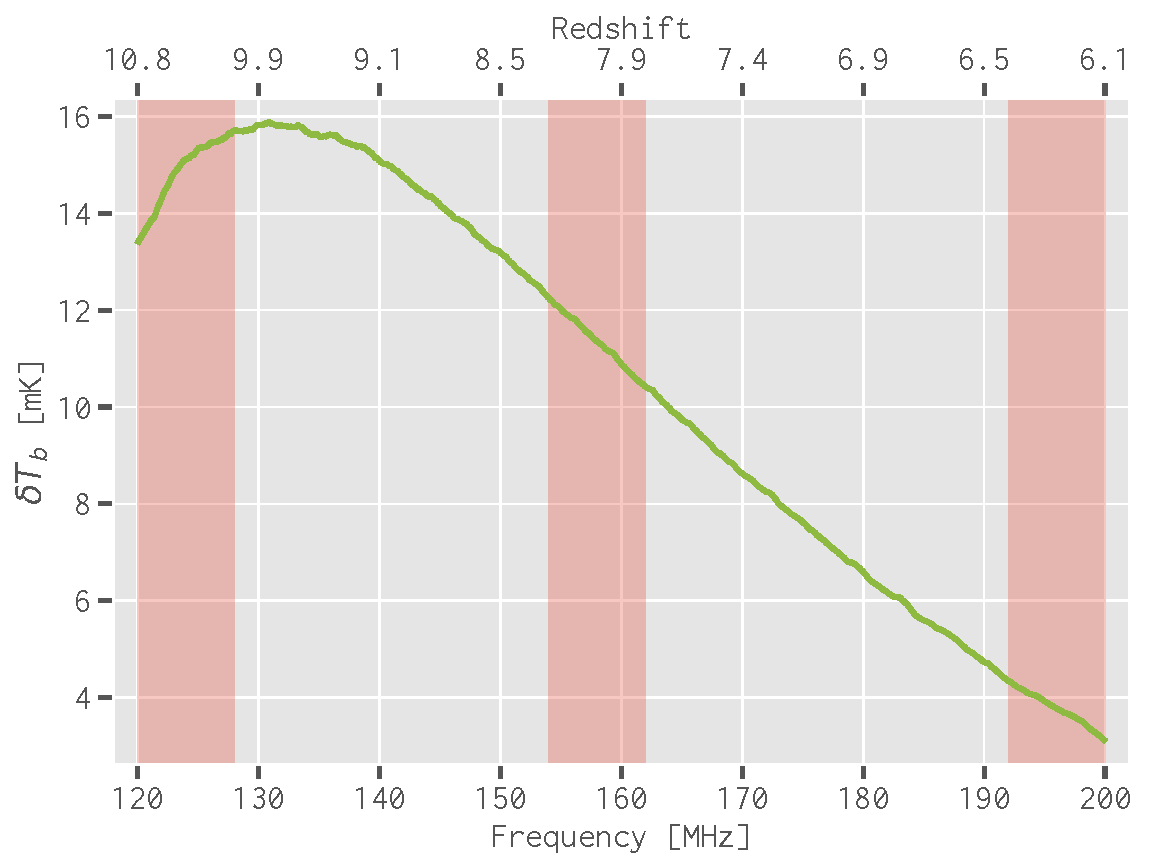
\includegraphics[width=0.8\textwidth]{eos2016-tbrms}
  \bicaption[EoR 信号在 \SIrange{120}{200}{\MHz} 的亮温度的\acs*{rms}值]{%
    EoR 信号在 \SIrange{120}{200}{\MHz} ($z = \numrange{6.1}{10.8}$)
    的亮温度的\acs*{rms}值(绿色实线).
    红色阴影区域表示本工作选取的三个频带:
    \numrange{120}{128}、
    \numrange{154}{162} 和 \numrange{192}{200} \si{\MHz}.
  }{%
    The root-mean-square brightness temperatures of the EoR signal
    (solid green line) within \SIrange{120}{200}{\MHz}
    ($z = \numrange{6.1}{10.8}$).
    The red shaded regions mark the three adopted frequency bands
    (\numrange{120}{128}, \numrange{154}{162}, and \numrange{192}{200}
    \si{\MHz}).
  }
  \label{fig:eor-tbrms}
\end{figure}

本工作使用了
\href{http://homepage.sns.it/mesinger/EOS.html}{\textit{Evolution Of 21\,cm Structure}}
项目\footnote{%
  Evolution Of 21\,cm Structure:
  \url{http://homepage.sns.it/mesinger/EOS.html}
} 公开的 EoR 模拟数据来生成所需的 EoR 信号的天图.
该项目使用
\href{http://homepage.sns.it/mesinger/DexM___21cmFAST.html}{\texttt{21cmFAST}}%
\footnote{%
  21cmFAST: \url{http://homepage.sns.it/mesinger/DexM___21cmFAST.html}
} 开展了宇宙再电离过程的高精度模拟,模拟盒子的边长为 \SI{1.6}{\Gpc},
划分为 1024 个单元,红移从 86.5 至 5.0 \cite{mesinger2016}.
\autoref{fig:eor-tbrms} 显示了 EoR 信号在 \SIrange{120}{200}{\MHz}
($z = \numrange{6.1}{10.8}$) 的亮温度的\acs*{rms}值.

利用该项目推荐的 \enquote{faint galaxies} 情形的\ac{lightcone} \ac{imgcube},
我们提取所需红移(即对应所需的频率)处的图像\ac{slice},
然后经过适当的平铺 (tile) 和缩放,使其图像大小为 \num{1800 x 1800}
以及天区覆盖为 \SI{10 x 10}{\degree}),即与前言的前景天图一致.
\autoref{tab:tb-rms} 中罗列了 EoR 信号在三个频带的中心频率处的亮温度的\ac{rms}值.
\autoref{fig:eor-skymap} 显示了 EoR 信号在 \SI{158}{\MHz} 的天图.

\begin{figure}[htp]
  \centering
  \includegraphics[width=0.7\textwidth]{skymap-eor-f158}
  \bicaption[EoR 信号在 \SI{158}{\MHz} 的天图]{%
    EoR 信号在 \SI{158}{\MHz} 的天图.
    天区的大小为 \SI{10 x 10}{\degree},
    \ac{colorbar}以 \si{\mK} 为单位.
  }{%
    The sky map of the EoR signal at \SI{158}{\MHz}.
    The sky region size is \SI{10 x 10}{\degree}
    and the color bar is in units of \si{\mK}.
  }
  \label{fig:eor-skymap}
\end{figure}


%=====================================================================
\section{干涉阵列的模拟观测}
\label{sec:obs-simu}

干涉阵列的复杂仪器效应是制约 EoR 探测的一个重要因素
(参见 \autoref{sec:det-difficulties}),
同时还会影响前景干扰的行为,比如导致\ac{fg-wedge}
(参见 \autoref{sec:eor-window}).
为了有效地评估射电晕对 EoR 探测的具体干扰情况,
整合干涉阵列的仪器效应是很有必要的.
为此,本工作采用了目前最新的 SKA1-Low 阵列布局\footnote{\raggedright%
  SKA1-Low 阵列布局坐标:
  \url{https://astronomers.skatelescope.org/wp-content/uploads/2016/09/SKA-TEL-SKO-0000422_02_SKA1_LowConfigurationCoordinates-1.pdf}
  (发布日期: 2016 年 5 月 31 日)},
对上文模拟得到的\ac{skymap}进行模拟观测,
获得整合了真实仪器效应的射电图像.

%---------------------------------------------------------------------
\subsection{SKA1-Low~阵列布局}

SKA1-Low 干涉阵列由 512 个\ac{station}组成,每个站点包含 256 根天线,
合计 \num{131072} 根天线.
每个站点呈直径 \SI{35}{\meter} 的圆形区域,
256 根天线保持最小间隔 $d_{\R{min}} = \SI{1.5}{\meter}$
随机分布其中 \cite{mort2017}.
512 个站点的布局方式分为两种情况 \cite{dewdney2016ska}:
\begin{itemize}
  \item 核心区域(半径 $R \le \SI{500}{\meter}$):随机分布 224 个站点;
  \item 核心区域之外:余下的 288 个站点构成 48 个站点团(每个团由 6 个站点组成),
    分布在 3 条半径达 $\sim$\,\SI{35}{\km} 的螺旋线上,
    形成长达 $\sim$\,\SI{65}{\km} 的基线.
\end{itemize}
\autoref{fig:ska1low-config} 显示了 SKA1-Low 的站点布局.
利用这种布局方式,一方面核心区域的大量短基线能够提供非常高灵敏度的 EoR 测量,
另一方面,长基线提供的高分辨率能够获得精确的前景模型,有利于 EoR 探测的前景扣除.

\begin{figure}[htp]
  \centering
  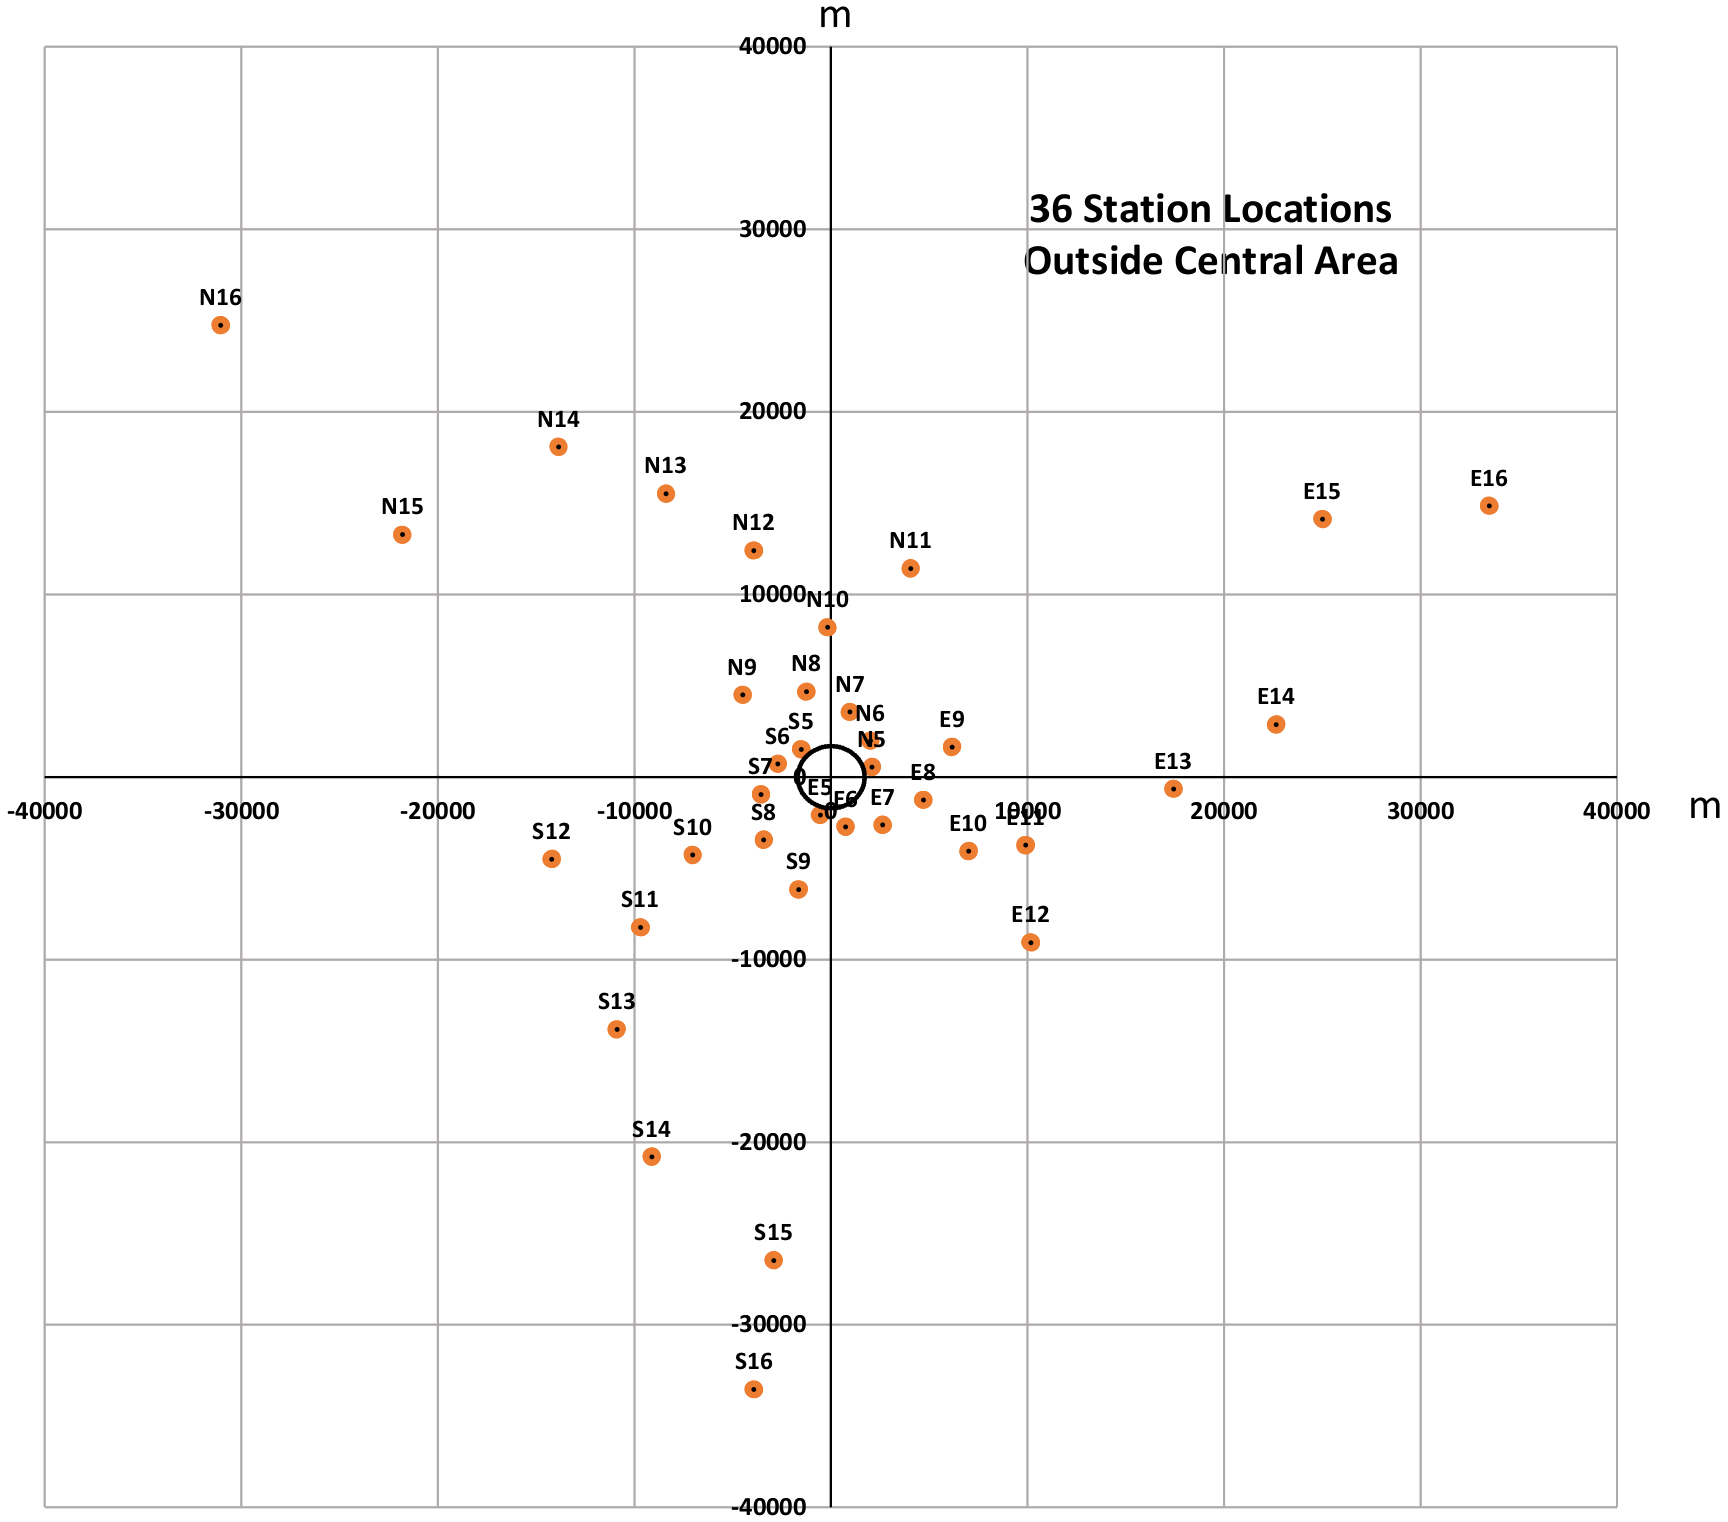
\includegraphics[width=0.508\textwidth]{SKA1low-config-outside}%
  \hfill%
  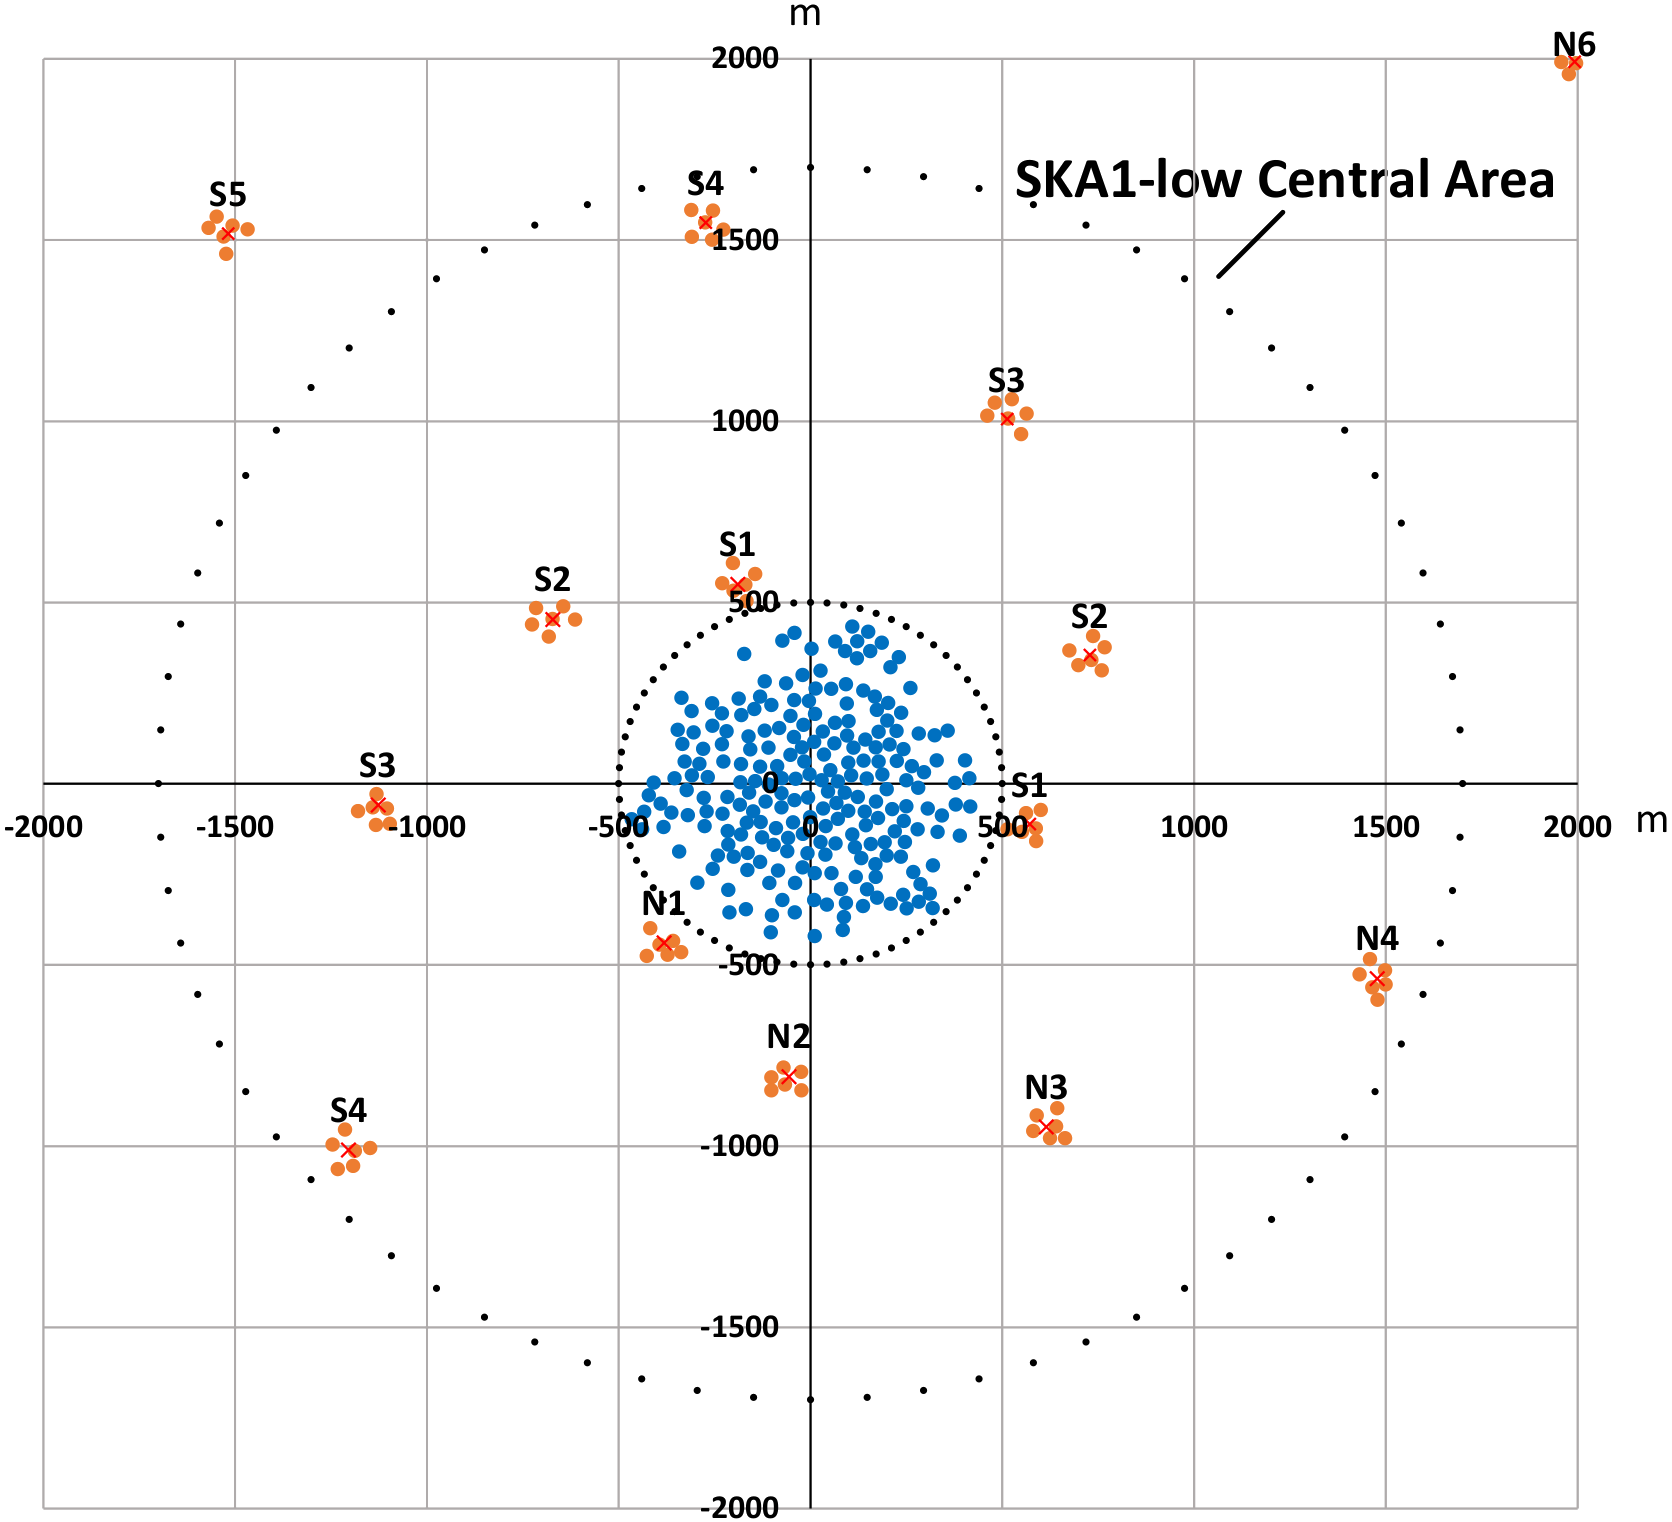
\includegraphics[width=0.491\textwidth]{SKA1low-config-central}
  \bicaption[SKA1-Low 站点布局图]{%
    \uline{(左栏)}
    中央区域 (半径 $R \le \SI{1700}{\meter}$) 之外的站点布局,
    由分布在 3 条螺旋线上的 36 个站点团 (station cluster) 构成,
    每个站点团包括 6 个站点.
    \uline{(右栏)}
    中央区域内的站点布局,
    包括核心区域 (半径 $R \le \SI{500}{\meter}$) 内随机分布的 224 个站点,
    以及 12 个分布在核心区域之外的站点团.
  }{%
    \emph{(Left)}
    The layout configuration of stations outside the central area
    (radius $R \le \SI{1700}{\meter}$).
    There are 36 station clusters, each of which consists of 6 stations,
    placing on 3 spiral arms.
    \emph{(Right)}
    The layout configuration of stations in the central area,
    including the 224 randomly distributed stations in the core area
    (radius $R \le \SI{500}{\meter}$) and another 12 station clusters
    outside the core area.
    \\来源/Credit:
    \citeay{dewdney2016ska}.
  }
  \label{fig:ska1low-config}
\end{figure}

%---------------------------------------------------------------------
\subsection{模拟观测和成像}

每一个 \SI{8}{\MHz} 的频带被分为 51 个频率\ac{channel},
对应的频率分辨率为 \SI{160}{\kHz}.
在每一个频率\ac{channel},首先模拟各个成分(包括前景辐射和 EoR 信号)的\ac{skymap},
然后使用 \href{https://github.com/OxfordSKA/OSKAR}{\texttt{OSKAR}}\footnote{%
  OSKAR: \url{https://github.com/OxfordSKA/OSKAR} (v2.7.0)}
模拟软件\cite{mort2010}
对每张\ac{skymap}进行模拟观测,积分时间为 \SI{6}{\hour},
获得\ac{vis}数据.
输入\ac{skymap}的中心被放置在
(R.A., Dec.\@) = (\SI{0}{\degree}, \SI{-27}{\degree}),
因为该点能够经过 SKA1-Low 的\ac{zenith},
是开展模拟观测的理想选择 \cite{liu2009ps,datta2010}.
所以,在一次 \SI{6}{\hour} 的模拟观测过程中,
输入\ac{skymap}的中心的\ac{hourangle}范围为 $[\SI{-3}{\hour}, \SI{3}{\hour}]$.

因为银河系的\ac{rad-syn}和\ac{rad-ff}都是弥散型辐射,
而且后文的分析中并不区分两者,所以我们将这两个成分的\ac{skymap}叠加之后
再进行模拟观测.
在干涉阵列的实际数据处理流程中,其中的一个重要的步骤是实时校准并扣除明亮点源,
即\ac{src-peeling} \cite{noordam2004,mitchell2008,intema2009},
能够有效地提高图像的质量和\ac{dynamic-range}.
据此,我们假定 \SI{158}{\MHz} 流量密度 $S_{158} > \SI{50}{\mJy}$ 的河外点源
已从\ac{skymap}上移除 \cite{liu2009ps,pindor2011,mort2017}.
处理后的河外点源在 124、158 和 196 \si{MHz} 的亮温度的\ac{rms}值显著减小至约
\num{22.5e4}、\num{9.81e4} 和 \num{4.75e4} \si{\mK}.

模拟获得\ac{vis}数据后,接着再使用
\href{https://sourceforge.net/p/wsclean}{\texttt{WSClean}}\footnote{%
  WSClean: \url{https://sourceforge.net/p/wsclean} (v2.6)}
成像软件\cite{offringa2014}
生成相应的观测图像.
该软件实现了 \ac{w-stack} CLEAN 成像算法,适用于低频大视场成像,
已在 \ac{lofar} 和 \ac{mwa} 等项目中被广泛使用 \cite{offringa2014,offringa2017}.
本工作采用了 Briggs 权重\cite{briggs1995}
并且设稳健参数 (robustness) 为 0,
如此兼顾了成像的噪声水平和空间分辨率 \cite{briggs1995}.
图像的边缘区域会因为 CLEAN 程度不足而质量较差,
因此我们只切取图像质量较好的中央区域用于后文的分析.
考虑到望远镜的\acl{Fov}反比于观测频率 ($\ac{Fov} \propto \nu^{-1}$),
图像的切取大小在 \numrange{120}{128}、\numrange{154}{162} 和
\numrange{192}{200} \si{\MHz} 三个频带内分别为
\SI{6 x 6}{\degree}、\SI{5 x 5}{\degree} 和 \SI{4 x 4}{\degree}.

\begin{figure}[htp]
  \centering
  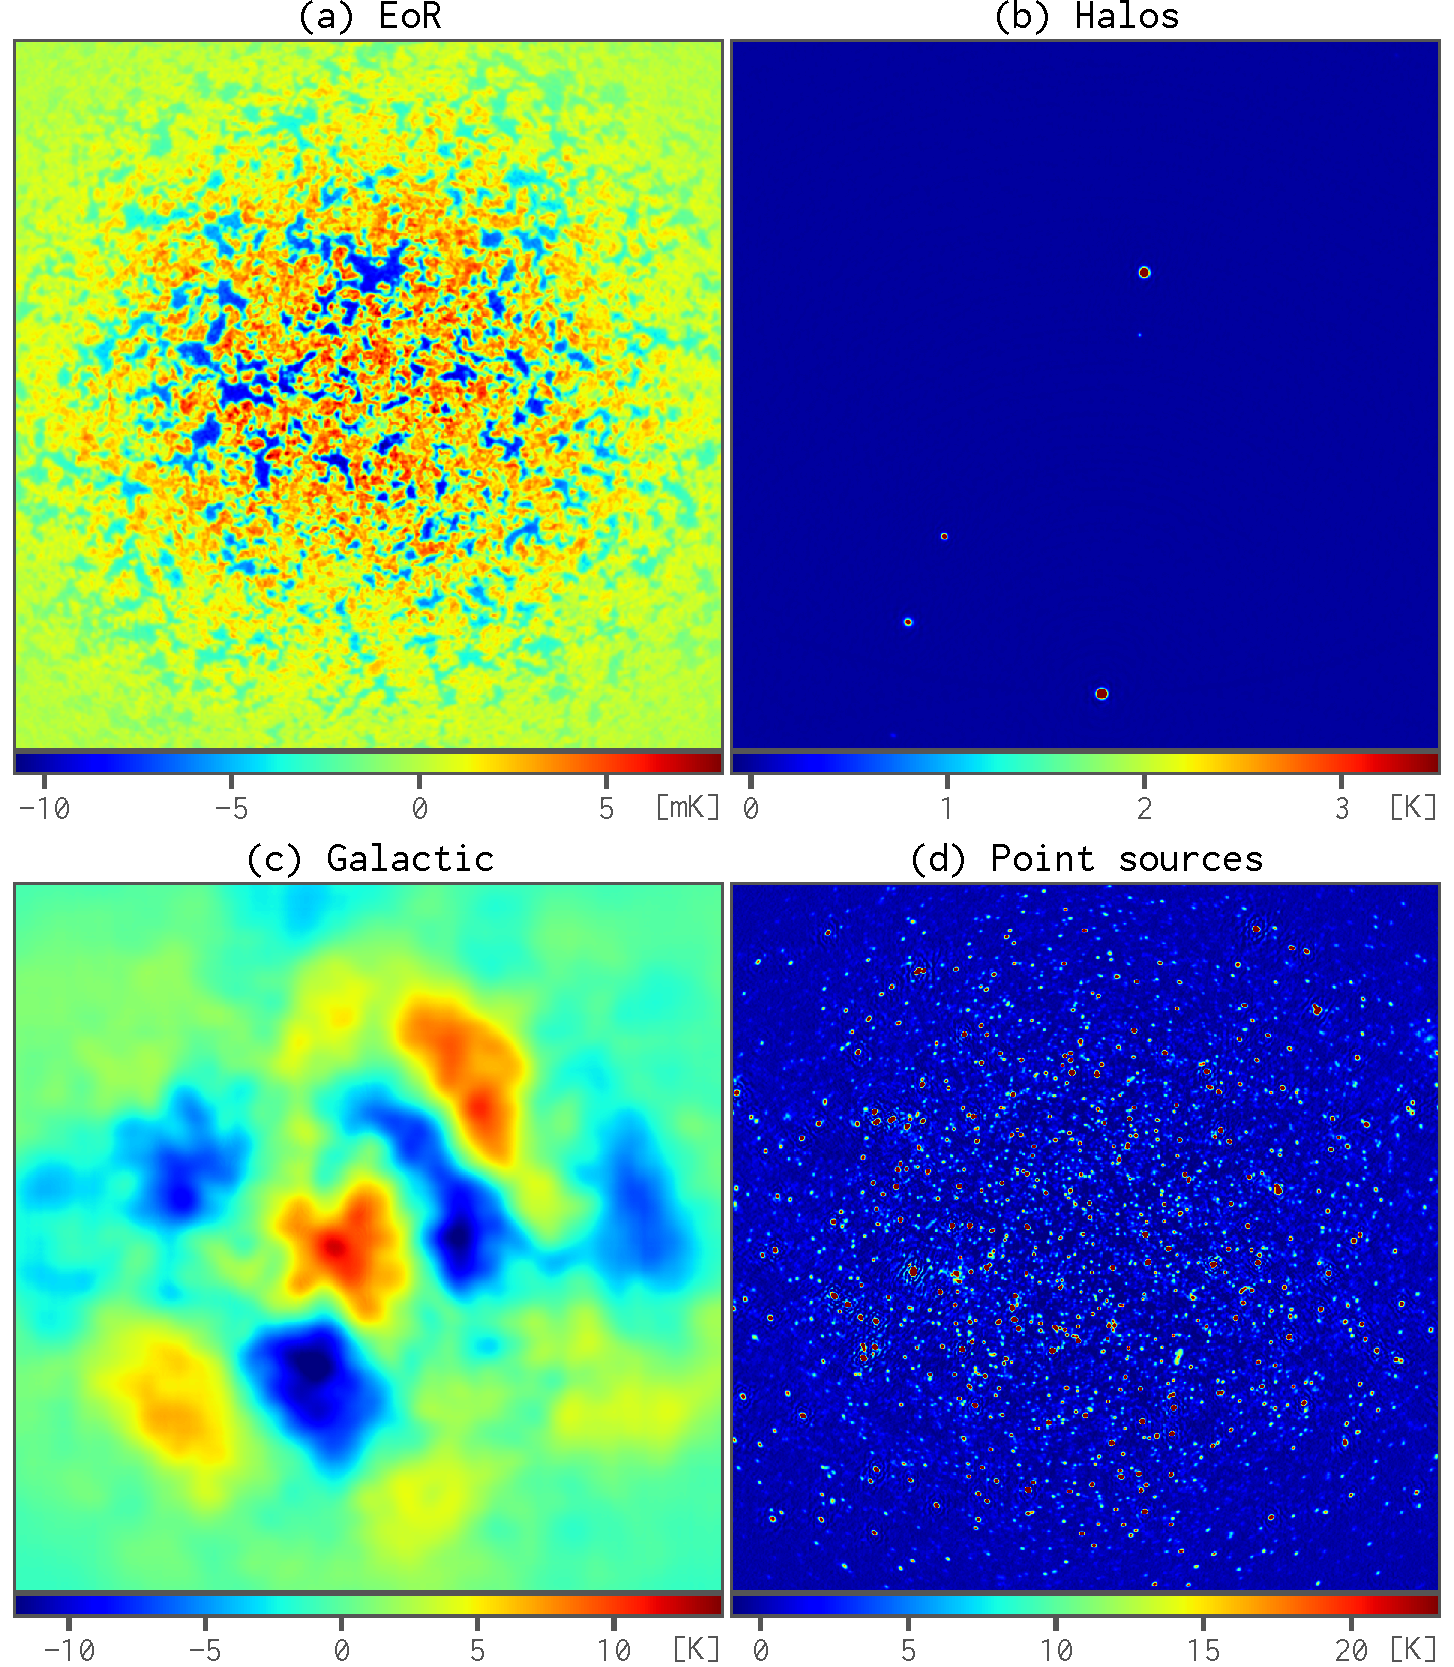
\includegraphics[width=\textwidth]{obsimg-all-f158}
  \bicaption[各成分在 \SI{158}{\MHz} 的模拟观测图像]{%
    各成分在 \SI{158}{\MHz} 的 SKA1-Low 模拟观测图像.
    从左上至右下分别为:
    \emph{(a)} EoR 信号;
    \emph{(b)} 射电晕;
    \emph{(c)} 银河系弥散辐射;
    \emph{(d)} 河外点源.
    所有图像覆盖的天区大小均为 \SI{10 x 10}{\degree},未经切取中央区域.
  }{%
    The simulated SKA1-Low observed images of all components
    at \SI{158}{\MHz}.
    From upper-left to bottom-right:
    \emph{(a)} EoR signal;
    \emph{(b)} radio halos;
    \emph{(c)} Galactic diffuse emission;
    \emph{(d)} extragalactic point sources.
    All the images cover a sky region of \SI{10 x 10}{\degree},
    without cropping out the central regions.
  }
  \label{fig:obsimg-all}
\end{figure}

前景的频谱光滑性是区分前景污染和 EoR 信号的关键.
为了保证这一点,我们利用了 \texttt{WSClean} 的联合\ac{channel}\ac{deconv}
(joined-channel deconvolution) 技术 \cite{offringa2017},
将一个前景成分(如射电晕)在一个频带(如 \SIrange{154}{162}{\MHz})
内 51 个\ac{channel}的\ac{vis}数据作为一个整体处理,得到相应的\ac{imgcube}.
由于 CLEAN 算法对 EoR 信号这种非常暗弱的弥散辐射处理效果有限,
我们直接使用由 \texttt{WSClean} 生成的\ac{dirty-map}.
尽管如此,因为 EoR 信号的\ac{skymap}中没有明亮的点状结构,
所以\ac{dirty-map}的质量已经足够好了.
这样,我们模拟得到了以下成分在 \numrange{120}{128}、\numrange{154}{162}
和 \numrange{192}{200} \si{\MHz} 三个频带内由
SKA1-Low \enquote{观测}得到的\ac{imgcube}:
\begin{itemize}
  \item EoR 信号;
  \item 银河系弥散辐射(包括\ac{rad-syn}和\ac{rad-ff});
  \item 射电晕;
  \item 河外点源.
\end{itemize}
\autoref{fig:obsimg-all} 展示了各成分在 \SI{158}{\MHz} 的模拟观测图像.


%=====================================================================
\section{小结}

TODO


%% EOF
